\chapter{Hidden Operating System (O/S)}

\section{MINIX O/S inside Intel's chip}

"Intel chipsets for some years have included a Management Engine [ME], a small
microprocessor that runs independently of the main CPU and operating system.
Various pieces of software run on the ME, ranging from code to handle media DRM
to an implementation of a TPM. AMT [Active Management Technology] is another
piece of software running on the ME."

In May 2017, AMT had a major security flaw, which had been in there for nine --
count 'em -- nine years.
\begin{itemize}
  
  \item  Fixing this requires a system firmware update in order to provide new
  ME firmware (including an updated copy of the AMT code)
  
  \item As many of the machines, which no longer receiving firmware updates from
  their manufacturers, and so will probably never get a fix, if AMT is enabled.
  
\end{itemize}
 
Ronald Minnich, a Google software engineer, who discovered a hidden MINIX
operating system inside "kind of a billion machines" using Intel processors.
These processors are running a closed-source variation of the open-source MINIX
3. It is a separate processor that is embedded in the motherboard chipset on
computers with Intel central processing units. It was introduced in 2005.
\begin{enumerate}
  
  \item  Intel's Management Engine is used for local and remote system
  management, which can be performed out of band even when the computer is
  turned off.
  
  This firmware runs on MINIX O/S. 
  ME has full access to the computer's system memory as well as network adapters.
  
  However, the typical operating system cannot access ME.
  
  "Based on the items identified through the comprehensive security review, an
  attacker could gain unauthorised access to the platform, Intel ME feature, and
  third party secrets protected by the ME, Server Platform Service (SPS), or
  Trusted Execution Engine (TXE)," the chipmaker said.
  
\end{enumerate}



We don't know exactly what version or how it's been modified since we don't have
the source code. We do know that with it there:
\begin{enumerate}
  \item  Neither Linux nor any other operating system have final control of the x86 platform Intel's ME.
  
  \item Between the operating system and the hardware are at least 2$\frac{1}{2}$ OS kernels (MINIX and UEFI)
  
  \item These are proprietary and (perhaps not surprisingly) exploit-friendly

  \item The exploits can persist, i.e. be written to FLASH, and you can't fix that
  
  \item Intel's ME is running on three separate x86 cores on modern chips. 
  
  \item Intel's ME also has access to your passwords. It can also reimage your
  computer's firmware even if it's powered off, but still plugged in, i.e. Intel's ME can
  still potentially change your computer's fundamental settings.
  
  It "can implement self-modifying code that can persist across power cycles".
  So, if an exploit happens here, even if you unplug your server in one last
  desperate attempt to save it, the attack will still be there waiting for you
  when you plug it back in.
  
  Intel's ME can do all this because the operating-system it runs on, i.e.
  MINIX, runs at a fundamentally lower level.
  x86-based computers run their software at different privilege levels or
  "rings".
  The lower the number your program runs at, the more access they have to the
  hardware
  \begin{itemize}
    \item  Your programs run at ring three, and they have the least access to the hardware
    
    \item Operating systems run on ring zero. 
    
    \item Bare-metal hypervisors, such as Xen, run on ring -1.
    
    \item  Unified Extensible Firmware Interface (UEFI) runs on ring -2
    
    \item MINIX? It runs on ring -3.
  \end{itemize}
  
  
  \item 
\end{enumerate}
\url{https://www.zdnet.com/article/minix-intels-hidden-in-chip-operating-system/}

In 1987, Tanenbaum wrote a clone of UNIX, called MINIX (MINi-unIX), for the IBM PC. 


Another aspect why using MINIX is bad, i.e. they should switch to using open-source Linux-based firmware.
\begin{itemize}
  
  \item  According to Minnich, booting an Open Compute Project (OCP) Server
  takes eight minutes thanks to MINIX's primitive drivers. With Linux it would
  take less than 17 seconds to get to a shell prompt. That's a speedup of 32
  times.
  
  "There are probably 30 million-plus Chromebooks out there and when your
  Chromebook gets a new BIOS, a new Linux image is flashed to firmware and I
  haven't heard of any problems."
  
  \item 
  
  
\end{itemize}


\chapter{Linux Kernel}

\section{Design concepts}


\begin{framed}
3 major kernel architectures:
\begin{enumerate}
  \item microkernel ($\mu$-kernel, Samuel kernel): use the minimum amount of
  software just to provide the enough mechanisms to implement an OS. They
  include low-level address-space mangement, thread management, and
  inter-process communication (IPC). Typically, a microkernel has $< 10,000$
  line of source codes. Other things run at user-mode.
  \item monolothickernel: the entire OS works in kernel-mode. Device
  drivers can be added to the kernel as modules.
  \item hybrid kernel (macrokernel): like Windows NT family (Windows 8, Windows
  Server 2012)
\end{enumerate}
When address space switches from 16-bit to 32-bit, kernels began to grow. BSD
UNIX pioneered the era of big kernels, giving kernels with millions of code
lines, e.g. Linux 3.10 kernel has about 16 millions lines of code.
\end{framed}

\subsection{UNIX vs Unix?}

{\small
\begin{verbatim}
Some people are confused over whether this word is appropriately
    `UNIX' or `Unix'; both forms are common, and used interchangeably.
    Dennis Ritchie says that the `UNIX' spelling originally happened
    in CACM's 1974 paper "The UNIX Time-Sharing System" because "we
    had a new typesetter and troff had just been invented and we were
    intoxicated by being able to produce small caps." Later, dmr tried
    to get the spelling changed to `Unix' in a couple of Bell Labs
    papers, on the grounds that the word is not acronymic. He failed,
    and eventually (his words) "wimped out" on the issue. So, while
    the trademark today is `UNIX', both capitalizations are grounded
    in ancient usage; the Jargon File uses `Unix' in deference to
    dmr's wishes.
\end{verbatim}
}

\url{http://www.luci.org/luci-discuss/200104/msg00031.html}


\subsection{UNIX kernel concept}


UNIX concept: everything-as-a-file, which is might not be fast enough on modern
systems.
The critical abstraction of UNIX was the {\bf pipe}, i.e. a set of processes
chained by their standard streams so that the output (stdout) of one process
feeds directly to the input (stdin) of the next one. The shell syntax for a
pipe:
\begin{verbatim}
program1 | program2 | program3
\end{verbatim} 
By default, the standard error (stderr) is not passed through the pipe (instead, they are merged 
and directed to the console). To force direct the standard error to the pipe, use
\verb!2>&1! in Bourne shell (and related shells: bash) or \verb!|&! (instead of \verb!|!) in csh shell.

\subsection{Accent kernel concept}
\label{sec:Accent-kernel_concept}

Accent kernel project: built IPC (inter-process communication) - something like
pipe, but allows a broad variety of information to be passed between programs,
as apposed to file-like information in UNIX.
However, Accent is not UNIX-compatible.


\subsection{Mach microkernel}
\label{sec:Mach_kernel}

{\bf Mach} is a kernel to support O/S research, primarily distributed
and parallel computation. The project ended with Mach 3.0 (1994)
which is finally a true microkernel.

O/S based on Mach
\begin{itemize}
  \item NeXTSTEP
  \item OS X
\end{itemize}

Mach design concept: bring Accent-concept
(Sect.\ref{sec:Accent-kernel_concept}) to UNIX, and works well on parallel
systems. From that, a number of generic concepts were developed
\begin{itemize}
  \item {\bf task}: an object consisting a set of system resources that enable
  threads to run
  
  A task is a process, i.e. which can consist a number of threads. 
  This is nowadays a common concept in modern O/S.
  
  \item {\bf thread}: a single unit of execution (exists within the context of a task, 
  and share task's resources)
  
  \item {\bf port}: a protected message queue for communication between tasks
  
  \item {\bf messages}: a collection of typed data objects, and can only be sent to ports
  - not specifically tasks or threads.
\end{itemize}
A {\bf port} represents each endpoint of a two-way IPC. Ports had security and rights 
like files in UNIX. Like UNIX, Mach uses the concept of drivers for handling hardware
and all the drivers must be included in the microkernel. Exokernels move the drivers
out of the kernel (Sect.\ref{sec:exokernel})

\textcolor{red}{The main difference with UNIX is that instead of utilities handling files, they
can handle any "task".} Thus, more code, previously part of the O/S, is moved into the user-space,
resulting in a much smaller kernel - giving them the term {\bf microkernel}.
The kernel is no longer an O/S, i.e. it only does the jobs of maintaining a
set of utilities and scheduling their access to the hardware.

\subsection{exokernel}
\label{sec:exokernel}


NOTE:


\subsection{rings (CPU modes)}

To improve fault tolerance, a hierachical protection domain approach is used.
Here, the security levels are divided into rings, e.g. ring0 to ring3. This is
aka CPU modes.

The kernel runs at ring0 level which has the most provileged (access to anything
in the system - hardware + software). An outer ring can access an inner ring
(lower number) via some gates/interfaces. Hardware access, e.g. turning on the
webcam is on ring1 (with functions reserved for device drivers). A normal
software (e.g. spyware) can only run on ring3.

Windows 7 and Windows Server 2008 only has 2 rings: ring0 = kernel mode and
ring3 = user mode. The reason is that some old hardwares only implement two
privilege levels.

Even CPUs support more than 2 levels, but ring1 and ring2 are rarely used.

\section{Kernel patch/update}
\label{sec:kernel-update}

Traditionally, updating a kernel requires system reboot.
The reason is that every running process integrates with the kernel intimately,
so switching out parts of the kernel while it is running is quite risky.

To enable \verb!no-reboot! kernel patch,
\begin{itemize}
  
  \item Oracle has Ksplice - Sect.\ref{sec:Ksplice}
  
  \item RedHat developped \verb!kpatch! (Sect.\ref{sec:kpatch}) and 
  
   \item SUSE developped \verb!kGraft! (Sect.\ref{sec:kGraft}). 
\end{itemize} 

Since October 2014, the two companies unified the system and worked on no-reboot
kernel for Linux kernel 4.0+.
\url{http://www.linuxjournal.com/content/no-reboot-kernel-patching-and-why-you-should-care}

\subsection{Livepatch service Ubuntu}

Ubuntu 16.04 first provided livepatch service. Later, if Ubuntu 14.04, with
update to Linux kernel 4.4, can also receives livepatch service.
\begin{verbatim}
sudo snap install canonical-livepatch
\end{verbatim}


Ubuntu provides Canonical Livepatch service 
\begin{itemize}
  \item user needs to register with Ubuntu One (Sect.\ref{sec:Ubuntu-One})
  
  to get live-patch token and enable it
\begin{verbatim}
sudo canonical-livepatch enable <token-here>
\end{verbatim}
a single token can be used for up to 3 machines.  
  
  \item check status
  
\begin{verbatim}
 canonical-livepatch status
\end{verbatim}
\end{itemize}

\subsection{Ubuntu One}
\label{sec:Ubuntu-One}

\url{https://login.ubuntu.com/ssh-keys}

Register your machine \verb!~/.ssh/id_rsa.pup! 

Once you have your account setup, configure your \verb!snap!
(Sect.\ref{sec:snap})
\begin{verbatim}
sudo snap login youremail_id@us.ibm.com
\end{verbatim}



\subsection{kPatch (RedHat)}

Kpatch uses \verb!ftrace!

Kpatch does similar to Ksplice, i.e. it freezes the kernel and inspect its
state. Kpatch waits until all kernel-level function calls have stopped, then
swaps in the new kenel.
By doing that, kpatch needs to freezes every process and then reroutes system
calls from the old kernel functions to the new, patched functions, before
removing the old code. 

Because it handles every running process in one sweeping move, it runs quite
fast - one to forty milliseconds and it's done.
However, during this time the processes are frozen, which means there is some
downtime - a mere fraction of a second, but in certain situations, that may be
unacceptable, e.g. in banking.

\subsection{kGraft (SUSE: no down-time) since 2014}

kGraft also uses \verb!ftrace!

kGraft was released in 2014 for SUSE by Kosina.
\url{https://lwn.net/Articles/734765}

kGraft, on the other hand, uses a lazy approach, i.e. slowly migrate all
processes to use the new code. It handles each thread one by one, as they make
system calls (without forcing them to freeze first) until all of the threads are
running the patched code. At this point, the patch is fully installed and the
old code is replaced. This process takes longer to complete the patch, but it
does it without any downtime.    



\subsection{Ksplice (Oracle) - since 2008}
\label{sec:Ksplice}

\verb!Ksplice! was the first implementation of live patching for Linux kernel
(started as the code for PhD thesis since 2008, and then released open-source).
It was acquired by Orale in 2011, and the source code was closed - for Oracle
Linux. Each ksplice-enabled kernel has a special flag to each function that will
be patched.

It allows patching kernel without reboot the system. This is critical to many
servers. The strategy of Ksplice is to freeze the execution of the computer, so that
Ksplice is the only one running. 
It uses \verb!stop_machine()! function to stop the kernel, then inspect the
stack to see if the patch would interfere with any task currently running.
If the kernel-level function is found on any stack, ksplice refused to patch it
and retry later.

Ksplice also does binary comparison of original kernel and patched kernel; but
this is hard due to function inlining and other optimizations.

It then verifies that no CPU in in the middle of executing functions that will be updated by the patch. Then, Ksplice
modify the address pointing to the beginning of the changed function to the new,
updated version of the function, and modify related data structure in memory.

This limits to patches that don't have semantic changes to data structures.

\section{BSD/Ubuntu/\ldots}

The first UNIX OS was developed by AT\&T Bell's Lab in 1969. AT\&T later
licensed the development to vendors, i.e. they received free UNIX system code,
leading to various UNIX-variants, including Berkeley UNIX, HP-UX, AIX and
Microsoft's Xenis. 

In 1993, AT\&T sold the right of UNIX to Novell, Inc. and then a few years
later, it was sold again to one consortium later became {\it The Open Group}
(Sect.\ref{sec:UNIX-war}). UNIX OS was developed using C language, giving it
the portability to run on different hardware platforms.

{\bf BSD} (Berkeley Software Distributions) is a UNIX-based OS, developed and
maintained by UC Berkeley from 1977 to 1995. Another major variant of UNIX is
{\bf UNIX System V} which is he first commercial version of UNIX OS, developed
by AT\&T. There are 4 major release of System V: release 1, 2, 3, and 4. 

NOTE: System V release 4 (SVR4) is the most popular release. AT\&T sell the
hardware and publish the interface so that other companies can develop the
operating systems to interact with the hardware. These systems are developed by
big companies, e.g. AIX, Solaris and HP-UX. AIX is based on SVR3, while Solaris
and HP-UX are based on SVR4. {\it Solaris (Oracle), AIX (IBM) and HP-UX},
together, form the most popular variants of UNIX OS. They are widely used in
servers (due to high security), and workstations as it works extremely well for
multi-user environment, laverage the power of symmetric multiprocessing in
systems with \verb!>! 8 cores.

Other than proprietary UNIX-like OSs, there are free UNIX-like OSs: FreeBSD,
OpenBSD. OS-X from Apple is also a UNIX-based OS as it uses FreeBSD, with the
proprietary GUI shell called Acqua. FreeBSD (started 1993) is the most widely
used BSD-derived OSs. FreeBSD can run on different hardware architectures.

In 1991, Linus Tovarlds developed a Linux kernel (Sect.\ref{sec:kernel}) based
on Minix (UNIX-like OS) to target Intel x86-based chips, and made the source
code available under GNU GPL with the name Linux. The first Linux kernel 0.01
was compiled with GNU C compiler, and it has GNU's Bash shell. Linux is
POSIX-compliant, a family of standards (API, command-line shells, utility
interfaces, etc.) developed by IEEE to maintain compatibility between different
OSs. A UNIX-like OS must have
\begin{enumerate}
  \item a kernel: provide driver to control the hardware, handle memory
  management, system calls, and low-level functions commons to most programs
  \item With the kernel, a working system needs a shell, compilers, and libraries, etc.
  \item file system: a hierarchical directory structure, e.g. root (/), binaries
  used by all users (/bin), binaries used by normal users (/usr/bin), local
  configuration (/etc), shared libraries needed to boot the system and
  run the commands in root file system (/lib), static and shared libraries
  and few executables not invoked directly and subdirectories for complex
  programs (/usr/lib), spaces for temporary files (/tmp), etc.
\end{enumerate} 

The first POSIX version was released in 1988 (IEEE 1003 or ISO/IEC 9945.) POSIX
for UNIX-like OS started with a single page, and then grow into 19 separate
documents (POSIX.1, POSIX.2, etc.). In 2008, they were combined into a single
standard: IEEE Std 1003.1-2008, also known as POSIX.1-2008. Since 2009, a new
part is added:
\begin{enumerate}
  \item POSIX.1-2008: 
  \item POSIX Conformance Testing: a test suite 
\end{enumerate}

Linux was then ported to other hardware architectures. Thus, Linux is getting
more popular, particularly in medium-sized business.
However, as UNIX-based systems are so expensive (mid-range UNIX-based servers
cost 25K-250K including hardware, or more). The reason is that each UNIX system
is custom written for the client.
More companies are switching to Linux. In addition, Linux kernels are widely
used in embedded systems, and mobile platforms (Android). Server systems based
on Linux kernels: {\it RedHat, Mandrake, SUSE, Ubuntu}, etc. There are many many
other free distributions, with customized software packages for different
purposes, e.g. for education.

A Linux distribution include Linux kernel, supporting utilities and libraries.
The UI is based on either GNOME or KDE, or less resource-intensive desktop like
LXDE or Xfce. We don't need the UI if the system is designed to run on server,
which then may need to add software like LAMP. 



\subsection{Securities}

Even though UNIX and Linux-based OSs are also vulnerable to malware and
exploitations; both are more secure than Windows OSs. However, Linux are a
little more secured than UNIX as it's open source and the flaws can be easily
detected and fixed.



\section{Linux kernel version}
\label{sec:Linux_kernel}
\label{sec:kernel}

To check what kernel versions are available on your machine
\begin{verbatim}
find /boot/vm*  -printf "%A@ %p\n"
\end{verbatim}
RESULT:
\begin{verbatim}
1516651996.0000000000 /boot/vmlinuz-3.13.0-139-generic
1519889380.0000000000 /boot/vmlinuz-4.4.0-112-generic
1519914723.0000000000 /boot/vmlinuz-4.4.0-116-generic
\end{verbatim}
NOTE: \verb!w.xx.y-zzz! means
\begin{enumerate}
  \item \verb!w! = the version
  
  \item \verb!xx! = major revision 
  
  \item \verb!y! = minor revision 
  
  \item \verb!zzz! = ABI number (patch number) - Sect.\ref{sec:ABI}
\end{enumerate}
\url{https://askubuntu.com/questions/843197/what-are-kernel-version-number-components-w-x-yy-zzz-called/843198}

The change in Linux kernel version 1.x and 2.x are major changes, with 2.6.x.y
is the latest. Especially, the major change from Linux 2.4 to Linux 2.6
(Sect.\ref{sec:kernel-change-2.4-to-2.6})

The jump to Linux kernel 3.x is not a major change, compared to
2.6, but to commenmorate the 20th anniversary of Linux.
The changelog:
\begin{itemize}
  \item 2.4: \url{https://www.kernel.org/pub/linux/kernel/v2.4/}
  
  NOTE: Linux-2.5.0 is exactly the same as 2.4.15
  
  \item 2.6: \url{https://www.kernel.org/pub/linux/kernel/v2.6/}
\end{itemize}
\url{http://kernelnewbies.org/Linux_3.12}

Check the location of an item (macro, struct) in which file: 
\url{http://lxr.free-electrons.com/ident?v=2.0.40;i=GFP_KERNEL}

The reason to choose a proper kernel version is if you're using Docker
(Sect.\ref{sec:Docker}).
In general, kernel 3.10 is the absolute minimum kernel version that supports the
features that Docker requires to run stable (newer versions are preferred
though).


Many kernel architectures in Linux-based OSs use the {\it loadable kernel
module} (LKM) approach (Sect.\ref{sec:LKM}). Instead of loading everything at
once during the boot, which many of the components may not be used which leads
to waste of resources. Using LKM, the {\it base kernel} has the minimum loaded
modules, and upon request, we can extend the features by loading more modules
using the commands: \verb!insmod! or \verb!modprobe! in Linux.

Compare performances of different kernel versions (from 3.5 to 4.4):
\url{https://www.phoronix.com/scan.php?page=article&item=linux-44-19way&num=1}

References:
\begin{itemize}
  \item 
\url{http://kernelnewbies.org/LinuxChanges}

  \item
\url{http://kernelnewbies.org/LinuxVersions}
\end{itemize}


\subsection{4.18 (Ubuntu 18.10)}
\label{sec:linux-kernel-4.18}

Ubuntu 18.10 switch to 
\begin{enumerate}
  \item Linux kernel 4.18
  
adds, among other things, support for AMD Radeon RX Vega M graphics processors, complete support for the Raspberry Pi 3B and the 3B+ models, and improved Thunderbolt and USB Type-C tweaks,

A reverse engineered Steam Controller driver also features as part of the mainline kernel. This lets the Steam Controller work as a regular HID (input) device ‘out of the box’, no Steam app required.

The latest Mesa 18.2 graphics drivers are included too, bringing a veritable gantry of improvements, including Vega GPU support, compatibility with OpenGL 4.4, and more.
  
  \item Update: GNOME 3.30
  
Better memory usage: GNOME Shell, 
  
  \item new icon sets
  
  Dubbed “Yaru”, the new theme is the work of the Ubuntu user community (and was known as the ‘Communitheme’ for a while). 
  
\end{enumerate}


\subsection{4.16}
\label{sec:linux-kernel-4.16}

The in-development Linux 4.16 kernel has already received a few rounds of
updates for the mitigation work on the Spectre and Meltdown CPU vulnerabilities
(Sect.\ref{sec:Meltdown})


This code also has more sanitization work, more robust microcode loading, using
IBRS (Indirect Branch Restricted Speculation) around firmware calls, objtool
support for Retpolines, and various other fixes/improvements.

\url{https://www.phoronix.com/scan.php?page=news_item&px=Linux-4.16-More-Spectre-Melt}


\subsection{4.15 (LTS Ubuntu 18.04)}
\label{sec:linux-kernel-4.15}

Ubuntu 18.04 switch to 
\begin{enumerate}
  \item Linux kernel 4.15
  
  \item OpenMPI 2.x by default
  
  \item CUDA 10.0 compatible
  
  \item GNOME 3.0
\end{enumerate}


\subsection{4.14 LTS (Nov.12-2017)}
\label{sec:HMM-heterogeneous-memory-management}

Since Linux kernel 4.14, the LTS support life cycle is 6 years.

The new release also features support for Address Space Identifier (ASID), AKA
as PCID on x86 systems, AMD memory encryption support for its EPYC processors,
and support for Intel's 5-level paging.

All this gives the latest Linux better memory management paging support for
virtual machines (VM)s. Specifically, virtualization programs such as Microsoft
Hyper-V, Xen, and KVM will work better with Linux 4.14. 

{\bf Heterogeneous Memory Management (HMM)} has also finally made it into Linux,
i.e. enables GPUs and CPUs to access a process's shared address space.
Both supercomputing and programs using parallel-processing languages and
application programming interfaces (API) such as OpenCL 2.0, Nvidia's CUDA, and
C++'s Parallel Algorithm Scheduling Library (PASL) will find this useful.  

\subsection{4.13 (Sept, 2017)}
\label{sec:linux-kernel-4.13}

Linux kernel 4.13 has mainly networking fixes (with various drivers). 

New features
\begin{enumerate}
  \item Initial Intel Cannonlake and Coffeelake CPU support
  
  \item Nouveau driver has HDMI 3D and stereoscopic support
  
  \item Radeon/AMD GPU DRM update
  
  \item new HID, audio hardware support
  
  \item new input drivers support
\end{enumerate}


\subsection{4.4 LTS (Jan 2016) - patch Meltdown}
\label{sec:linux-kernel-4.4}


It has more than 20.8 million lines of code.

Kernel 4.4.0-116 has patches for Metldown and Spectre
(Sect.\ref{sec:kernel-patch-Spectre}).

To get kernel 4.4. in Ubuntu 14.04. 
\begin{verbatim}
sudo apt-get install linux-generic-lts-xenial
\end{verbatim}

To update Ubuntu 14.04 completely, read Sect.\ref{sec:Ubuntu-14.04-upgrade}.

\url{https://insights.ubuntu.com/2018/01/04/ubuntu-updates-for-the-meltdown-spectre-vulnerabilities/}

\subsection{4.1 (June 2015)}

It has more than 19.5 million lines of code.

\subsection{3.14}

used by: Ubuntu 14.04


\subsection{3.13 (patch Meltdown)}


Linux 3.13 kernel has LTS, while the 3.16 and 3.19 kernels have shorter support
periods. Because of that, tThis is the only kernel in Ubuntu 

\subsection{3.11}

Improve performances and support more ARM architectures. 

\subsection{3.7}

Linux kernel 3.7 is the last one to support i386 processors. 


\subsection{2.6.26}

\begin{enumerate}

  \item new feature option: \verb!MODULE_FORCE_LOAD! 
  (which set to 'y' will enable the force loading a kernel module -
  Sect.\ref{sec:LKM})
  
  \item x86 CPU: use 8KB as the default stack size
  
  \item klist type:
  
  2 new functions: \verb!klist_add_after() and klist_add_before()!
  
  
  \item \verb!kmap_atomic_to_page()! is no longer exposed

\begin{verbatim}
---
f31eb5842f0a727041ff53355819cac964288428 diff --git a/arch/x86/mm/highmem_32.c b/arch/x86/mm/highmem_32.c
index 9cf33d3..165c871 100644
--- a/arch/x86/mm/highmem_32.c
+++ b/arch/x86/mm/highmem_32.c
@@ -155,4 +155,3 @@ EXPORT_SYMBOL(kmap);
 EXPORT_SYMBOL(kunmap);
 EXPORT_SYMBOL(kmap_atomic);
 EXPORT_SYMBOL(kunmap_atomic);
-EXPORT_SYMBOL(kmap_atomic_to_page);
\end{verbatim} 
\url{http://lists.openwall.net/linux-kernel/2008/04/21/116}

  \item new generic functions to perform 64-bit integer divisions: which
  specific signed or unsigned  math
  
\begin{verbatim}
 u64 div_u64(u64 dividend, u32 divisor);
    u64 div_u64_rem(u64 dividend, u32 divisor, u32 *remainder);
    s64 div_s64(s64 dividend, s32 divisor)
    s64 div_s64_rem(s64 dividend, s32 divisor, s32 *remainder);
\end{verbatim} 

which replace the old x86-specific function \verb!div_long_long_rem()!

   \item new string function: compare the two strings, but does not take into
   (i.e. ignore) the trailing newline input 

so 
\begin{verbatim}
> sysfs_streq("a", "a")	==> true
> sysfs_streq("a", "a\n")	==> true
> sysfs_streq("a\n", "a")	==> true
> sysfs_streq("a\n", "a\n") ==> true
\end{verbatim}

\begin{verbatim}
 bool sysfs_streq(const char *s1, 
                  const char *s2);
\end{verbatim}

which replaces the use of \verb!strcmp()!
\begin{verbatim}
-if (!strcmp(...))
+if (sysfs_streq(...))
\end{verbatim}
\url{http://permalink.gmane.org/gmane.linux.network/346631}


  \item I2C device: the prototype of \verb!probe()! change

\begin{verbatim}
 int (*probe)(struct i2c_client *client, 
                  const struct i2c_device_id *id);
\end{verbatim}
\url{https://www.kernel.org/doc/Documentation/i2c/instantiating-devices}

\end{enumerate}

\url{http://lwn.net/Articles/280647/}



\subsection{2.6.13}

Changes:
\begin{itemize}
  
  \item support: execute-in-place (better for embedded devices which store
  program in ROM/Flash chip (i.e. no need to copy to RAM and save page cache/io
  scheduler layer) vs. the traditional way - laoded from disk to memory to be
  executed)
  
  \item hotplug support (can be safely unregistering/registering procesors
  during runtime): i386
  
  \item new CPU architecture: Xtensa (embedded devices) 
  
\end{itemize}

\subsection{2.6.0}
\label{sec:kernel-change-2.4-to-2.6}

\url{https://wiki.gentoo.org/wiki/Kernel/Migrate_2.4_to_2.6}

The major change is the support of SMP architecture.
\url{https://www.ibm.com/developerworks/library/l-linux-smp/}


\subsection{2.5.18}

Changes: 
\begin{itemize}
  \item change: \verb!->getattr()->setattr()->permission()!
  \item support software suspend: disk and RAM  
\end{itemize}

\subsection{2.5.17}

Changes
\begin{itemize}
  \item ISDN4linux to CAPI based interface
  \item new quota system supporting plugins
\end{itemize}

\subsection{2.5.15, 2.5.16}

nothing 

\subsection{2.5.14}

Changes
\begin{itemize}
  \item support: Bluetooth (official), IDE TCQ (Tagged Command Queueing)
\end{itemize}

\subsection{2.5.12}

Changes: rewrite buffer layer	

\subsection{2.5.11}

Changes
\begin{itemize}
  \item rewrite: framebuffer layer
  
  \item fast walk dcache
  
  \item replace: NTFS old driver with NTFS TNG driver
\end{itemize}


\subsection{2.5.10}

nothing

\subsection{2.5.9}

Changes: smarter IRQ balancing	

\subsection{2.5.8}

Changes
\begin{itemize}
  \item radix-tree pagecache
  
  \item syscall interface for CPU task affinity
\end{itemize}

\subsection{2.5.7}

Changes
\begin{itemize}
  \item add: ACPI (Advanced Configuration and Power Interface)
  
  \item redesign: V4L (video 4 linux)
  \item new: driver API for Wireless Extensions
  \item mitigate: NAPI network interrupt
  \item use: Futexes (Fast Lightweight Userspace Semaphores) 
\end{itemize}

\subsection{2.5.6}

Changes
\begin{itemize}
  \item update: HDLC (High-Level Data Link Control)
  
  \item \verb!per_cpu! infrastructure
  \item add : JFS (Journalling FileSystem from IBM)
  
  \item 
\end{itemize}

\subsection{2.5.5}


Changes
\begin{itemize}
  \item support new hardware: ppc64, x86-64
  \item support: pageables in highmem
  
  \item add: ALSA (Advanced Linux Sound Architecture)
\end{itemize}

\subsection{2.5.4}

Changes
\begin{itemize}
  \item support: Next Generation POSIX Threading
  \item add: preempt kernel option
  \item change: user slabcache and sock.h for (1) per network protocol 
  and (2) per filesystem 
\end{itemize}

\subsection{2.5.3}

Changes
\begin{itemize}
  \item new driver model and unified device tree
  \item support: Generic Extended Attribute
  \item \verb!configure.help! is broken down into multiple files
  \item PnP BIOS driver
  \item \verb!sched.h! and \verb!fs.h! include dependencies
  \item update: IDE layer
\end{itemize}


\subsection{2.5.2}

Changes
\begin{itemize}
  \item initial support USB 2.0
  
  \item new kernel device structure \verb!kdev_t! in
  \verb!include/linux/kdev_t.h! file. This is a pointer to a structure with
  information about the device (e.g. major, minor, size, blocksize, sectorsize,
  name, read-only flag, struct \verb!file_operations!, \ldots)
  
  This type was introduced to hold a larger device numbers. Objects of this type
  designate a device and only known inside the kernel. Currently, outside of that,
  they are considered as objects of type \verb!dev_t!. It is upto the various filesystem
  to device how objects of type \verb!dev_t! are stored on disk.
  \url{https://www.kernel.org/pub/linux/kernel/people/akpm/patches/2.5/2.5.67/2.5.67-mm4/broken-out/64-bit-dev_t-kdev_t.patch}
  
  \item some improvement: O(1) scheduler, \ldots
\end{itemize}

\subsection{2.5.1}

It is the same as 2.4.15

\subsection{0.01 (yr 1991)}

The version 0.01 of the Linux kernel -- released in 1991 -- had just 10,239
lines of code.

\subsection{version}
\label{sec:Linux_kernel_version}

Check the current version of loaded kernel
\begin{verbatim}
$> uname -r
\end{verbatim}

\subsection{Keep one version and remove all the others}
\label{sec:Linux_kernel_keep-one-remove-others}

Suppose you have multiple kernels installed, and by default, the latest one is
used. If you want to use an older version, and remove all other others you don't
want to, you may need (1) disable automatic kernel update, (2) check which
kernel is being loaded (Sect.\ref{sec:Linux_kernel_version}), if not the one you
want to use then (3) follow these steps

How to : (suppose Ubuntu 10.04) and you want to use kernel 2.6.32-35-server
\begin{verbatim}
apt-get update
sudo apt-get install linux-image-2.6.32-35-server 
                 linux-headers-2.6.32-35-server
// restart
aptitude remove $(dpkg -l | egrep '^ii  linux-(im|he)' | 
      awk '{print $2}' | grep  -v `uname -r | awk )
// select proper option
update-grub2
// restart
\end{verbatim}

\subsection{namespaces in Linux kernel}
\label{sec:namespaces}

A Linux kernel has a number of namespace. Namespace and cgroups
(Sect.\ref{sec:cgroups}) are the two Linux processes that do resource
management.

Namespace provide {\it isolation}, i.e. enable a group of processes (one or
more) to have a different view of the system than other processes. It was first
used in {\bf Plan 9} distributed O/S in 1992
\url{http://www.cs.bell-labs.com/sys/doc/names.html}
It is much like Zones in Solaris. 
%A new system call \verb!setns()! was added. 

At Linux kernel 3.8, there are 6 different namespaces
\begin{enumerate}
  \item \verb!mnt! (mount point, filesystems)
  
  First appeared in Linux 2.4.19 in 2002, with \verb!CLONE_NEWNS! flag (stands
  for NEW NameSpace).   
  \item \verb!uts! (UNIX timesharing - hostname)
  \item \verb!ipc! (System V IPC)
  \item \verb!pid!
  \item \verb!net!
  
  \item \verb!user! (UIDS)
  
  User namespaces allow per-namespace mappings of user and group IDs.
  In Fedora 18 and Ubuntu 13.04, there is no
support for User Namespaces though it is kernel 3.8
  
\end{enumerate}
It is intended to have 10 namespaces, i.e. 4 have not been implemented yet
(security namespace, security keys namespace, device namespace, time namespace)

Check header file (there are more than 20 flags in total)
\begin{verbatim}
/include/linux/sched.h  

   ### flags
CLONE_NEWNS        Linux 2.4.19
CLONE_NEWUTS       Linux 2.6.19
CLONE_NEWIPC       Linux 2.6.19
CLONE_NEWPID       Linux 2.6.24
CLONE_NEWNEW       Linux 2.6.29
CLONE_NEWUSER      Linux 3.8
  \end{verbatim}
There are total 6 flags. To use any of the first 5 flags (i.e. not
\verb!CLONE_NEWUSER!) we need \verb!CAP_SYS_ADMIN! capability.

Three new system calls are added
\begin{itemize}
  \item clone()  : creata a new process and a new namespace (the process is
  attached to this namespace)

Also, the patch is required for existing process creation and process
termination functions (\verb!fork()! and \verb!exit()!) to handle the flags.

  \item unshare() : only create a new namespace, and attach this namespace to
  the current process
  
  It was added in 2005; but not only for namespace, but also for security
  
  \item setns() : not creating anything new, just allow the current process to
  join an existing namespace
\end{itemize}
The flags or any combination of them can be used in
\verb!clone()! and \verb!unshare()! syscalls to create a namespace.
It is optional in \verb!setns()! function.

The question is \textcolor{red}{How do we know if two processes in the same
namespace? }: There are six entries (inodes) added under 
\begin{verbatim}
/proc/<pid>/ns
\end{verbatim}
One for each namespace.

Example: 
\begin{verbatim}
 sudo ls -l /proc/18225/ns/
total 0
lrwxrwxrwx 1 root root 0 Jan 29 00:22 ipc -> ipc:[4026531839]
lrwxrwxrwx 1 root root 0 Jan 29 00:22 mnt -> mnt:[4026531840]
lrwxrwxrwx 1 root root 0 Jan 29 00:22 net -> net:[4026531956]
lrwxrwxrwx 1 root root 0 Jan 29 00:22 pid -> pid:[4026531836]
lrwxrwxrwx 1 root root 0 Jan 29 00:22 user -> user:[4026531837]
lrwxrwxrwx 1 root root 0 Jan 29 00:22 uts -> uts:[4026531838]
\end{verbatim}
\url{http://www.haifux.org/lectures/299/netLec7.pdf}


The structure \verb!nsproxy! in header file 
\begin{verbatim}
/include/linux/nsproxy.h
\end{verbatim}
contains pointers to all per-process namespaces
\begin{verbatim}
struct nsproxy {
     atomic_t count;
     struct uts_namespace *uts_ns;
     struct ipc_namespace *ipc_ns;
     struct mnt_namespace *mnt_ns;
     struct pid_namespace *pid_ns_for_children;
     struct net           *net_ns;
};
\end{verbatim}
\url{http://lxr.free-electrons.com/source/include/linux/nsproxy.h}


\subsection{cgroups}
\label{sec:cgroups}


Process Containers (launched by Google in 2006) was designed for limiting,
accounting and isolating resource usage (CPU, memory, disk I/O, network) of a
collection of processes. It was renamed “Control Groups (cgroups)” a year later
to avoid the confusion multiple meanings of the term “container” in the Linux
kernel context and merged to the Linux kernel 2.6.24.


In 2007: Control Groups merged into Linux kernel

When you run lots of containers on a system, you do not want to have any
container monopolize the operating system, so we use resource constraints to
control things like CPU, memory, network bandwidth, etc. The Linux kernel
provides the cgroups feature, which can be configured to control the container
process resources.


Redesign of cgroups started in 2013, with additional changes brought by versions
3.15 and 3.16 of the Linux kernel.


\verb!cgroups! (control groups) subsystem is a Resource Management solution
providing a generic process-grouping framework, which is considered better than
using the conventional process-id (PID) method - Sect.\ref{sec:init}).

The effort started by employees of Google in 2006 under the name {\bf process
container} and renamed to {\bf control group} in in 2007. It is used by
\verb!systemd! (Sect.\ref{sec:systemd}).

Note that the cgroups is not dependent upon namespaces; you can build cgroups
without namespaces kernel support.


The cgroup modules are not located in one folder but
scattered in the kernel tree according to their functionality
\begin{itemize}
  \item \verb!memory!  : mm/memcontrol.c
  \item \verb!cpuset! : kernel/cpuset.c
  \item \verb!net_prio! : net/core/netprio\_cgroup.c
  \item \verb!devices! : security/device\_cgroup.c
\end{itemize}

cgroups is recently supported in 
\begin{enumerate}
  \item kernel of Fedora 18 version
  \item kernel of Ubuntu 12.10 version
\end{enumerate}

Values in \verb!/proc/<pid>/cgroup!. Example:
\begin{verbatim}
2:name=systemd:/user/1000.user/1.session
\end{verbatim}

\subsection{Kernel driver}

A driver is a bit of code that runs in the kernel to talk to some hardware
device. It "drives" the hardware. Most every bit of hardware in your computer
has an associated driver. One exception to this broad statement is the CPU chip,
which has no "driver" per se. Your computer may also contain hardware for which
you have no driver.

Standard practice is to build drivers as kernel modules
(Sect.\ref{sec:kernel-modules}) where possible, rather than link them statically
to the kernel, since that gives more flexibility.

To list kernel drivers, we use \verb!lspci! (Sect.\ref{sec:lspci}).
\url{http://unix.stackexchange.com/questions/47208/what-is-the-difference-between-kernel-drivers-and-kernel-modules}
\section{Variants of Linux kernel}


Real-time kernel: \url{https://rt.wiki.kernel.org/index.php/Main_Page}

\url{http://lwn.net/Articles/146861/}

\url{http://www.linuxtopia.org/online_books/linux_kernel/kernel_configuration/ch09s03.html}

\subsection{Linux-libre}

A Linux-based OS typically include packages with no source-code available or
released under proprietary licenses. Packages with no source-code are known as
{\bf binary blobs}, and have been included in Linux kernel since 1996. These
include device firmware.

\verb!Linux-libre! is a variant that only include free software with source-code
available, and started since 2008. A script to remove binary blobs in called
{\bf deblob-main}. This make the OS lacks support for some hardware devices
like sound, video graphics, network cards, etc.

OS using \verb!linux-libre! as the kernel are gNewSense, Music GNU/Linux, etc.

\subsection{CNK and INK}

CNK and INK are lightweight kernels designed to run on nodes of supercomputers
(Sect.\ref{sec:kernel_IBM_BlueGene})

%\section{Tizen vs. Android vs. iOS}

\subsection{Tizen kernel}

Tizen use HTML5 to write apps. Android use Java, while iOS use Objective-C.

HTML5 enables smooth web browsing, e.g. display embeded video and music without
an additional plugins and no need to save data offline.

Tizen can be used not only on smartphones but in smart TV and many other smart
devices.

\subsection{Android kernel}

CyanogenMod: \url{https://github.com/CyanogenMod/cm-kernelspace}


\subsection{iOS kernel}


\subsection{minimax-linux}
\label{sec:minimax-linux}

Minimax is Linux distribution based on Linux 2.6 kernel and fits into 30MB
initrd image. It contained lot of command line tools and full Linux kernel. Was
based on UcLibc, Gentoo compilation and Squasfs.

\url{https://code.google.com/p/minimax-linux/}

\subsection{UEK (Unbreakable Enterprise Kernel)}
\label{sec:UEK-Unbreakable-Enterprise-Kernel}

Unbreakable Enterprise Kernel (UEK) is the heavily tested and optimized
operating system kernel for Oracle Linux.

Oracle Linux is application binary compatible with Red Hat Enterprise Linux
whether running the Unbreakable Enterprise Kernel or Oracle's alternative Red
Hat compatible kernel. The Oracle Linux operating system is engineered for open
cloud infrastructure.


\begin{enumerate}
  \item  
  
  \item 
\end{enumerate}


 

\section{Preemptive and Non-preemptive kernels}

An application can run in either modes: user-space-mode or kernel-mode (within
the kernel's memory space - executing a system call or having the kernel work on
behalf). This section is closely related to Chap.\ref{chap:parallelization}.

\subsection{non-preemptive kernel}
\label{sec:nonpreemptive-kernel}

In a non-preemptive kernel, a kernel-mode program can take the control of the
CPU forever.
Until Linux 2.6, the kernel is non-preemptive, i.e. the code running in kernel
keep using until it stops or it decides to allow the {\it scheduler} to run
another thread via the \verb!schedule()! function. Codes in kernel mode can not
be stopped (ignoring timeslices and important events). It means that the
scheduler can suspend processes running at user mode only; but
not able to suspend a process running in kernel
mode.\footnote{\url{http://www.itworld.com/nl/lnx_tip/11022001}}. Of course, the
kernel code is designed so that there is no infinite loop.

\subsection{(selective) preemptive-kernel}
\label{sec:preemptive-kernel}

In a preemptive kernel, if the running threads, regardless of the running mode,
takes the CPU for so long and does not voluntarily give up the CPU; the O/S
preempts it (Sect.\ref{sec:preemption}).
A preemptive kernel can suspend a process/thread running in kernel mode after
any instruction. In a preemptive kernel, each kernel function has a time slice
to use the resource (e.g. CPU). So, a process running in kernel mode can be
replaced by another process while in the middle of the function by the
scheduler.

\textcolor{red}{Linux kernels are indeed not fully preemptive}, as some critical
functions need to run without interruption. So, it's called {\bf selective preemptive kernels}.

Early version of preemptive kernel started by programmers at MontaVista. They
modified the definition of {\bf spin lock} (Sect.\ref{sec:spinlock}) to include
marking a ``non-preemptive'' region. On uniprocessor (UP) system, \verb!spin_lock! is
defined as \verb!preempt_disable! and \verb!spin_unlock! is defined as
\verb!preempt_enable!. They both operate on \verb!preempt_count! (a new integer
stored in each \verb!task_struct!).

Since Linux kernel 2.6, it supports preemptive option. In Linux 2.6, the
preemptive of the kernel can be turned on/off by modifying the feature
\verb!CONFIG_PREEMPT! option before compiling
(Sect.\ref{sec:build_Linux-kernel}).\footnote{\url{http://unix.stackexchange.com/questions/5180/what-is-the-difference-between-non-preemptive-preemptive-and-selective-preempti}}


\subsection{preemptive multitask with SMP}

With preemptive multi-tasking, lowering the latency when switching tasks in a
kernel is an important goal. 

Audio/video processing and playback are two common beneficiaries of lowered
latency. To avoid the delay for code running in kernel mode, the first and
simplest solution is to try to implement the kernel algorithm so that it takes
the minimum amount of time. The second is to insert explicit scheduling points
throughout the kernel. %The better solution is to make the kernel preemptive. 

The issue can be resolved by taking the advantages of SMP (symmetric
multiprocessing) support of newer hardwares. 


    
\subsection{Concurrency and race conditions}

Concurrency refers to the capability of a system doing more than one thing at
once. In early days of CPU architecture, it's uniprocessor, and concurrency is
achieved by {\bf task switching}, i.e. switching from one task to another using
hardware interrupts (Sect.\ref{sec:concurrency-programming}).

In systems with more than one processor, i.e. SMP (symmetric multiprocessing).
{\it preemption} was added to the kernel; so it is the job of the kernel to
switch one process to another; but not the job of the user-space programs.



\subsection{Preemption}
\label{sec:preemption}

``Preemption'' in computer science means that a running process/thread can be
suspended and giving the CPU for another thread to use. Typically, a running
thread is suspended once it has used the CPU for an alloted quantum, known as
{\it CPU timeslice}, to give the resouce to another one in the queue. Due to
different process priorities, the implementation of the scheduling is more
complicated.


\textcolor{red}{NOTE: This applies to processes running in kernel mode only}, as
under Linux, processes in user-mode are always preemptible, the kernel can
interupt based on regular clock tick. Since Linux kernel 2.6, the OS has the
ability to preempt or to stop a currently running task to schedule of a higher
priority task. 
With preemptive enabled, the kernel code can have {\it infinite} loop.




\section{I/O subsystem}
\label{sec:I/O-subsystem}

Without I/O, computers are not very useful. But there are thousands of devices,
each slightly different. So, how to standardize the interface to all devices?

\subsection{devices with different speed}

\begin{itemize}
  \item divices have different speed

\begin{verbatim}
DEVICES                          DATA RATE
--------------------------------------------
keyboard                  10 bytes/sec
mouse                    100 bytes/sec
56K modem                  7 KB/sec
scanner                  400 KB/sec
digital camcorder         3.5 MB/sec
802.11g wireless         6.75 MB/sec
52x CD-ROM               7.8  MB/sec
fast Ethernet            12.5 MB/sec
compact flash-card       40   MB/sec
Firewire (IEEE 1394)     50   MB/sec
USB 2.0                  60   MB/sec
SONET OC-12 network      78   MB/sec
SCSI Ultra 2 disk        80   MB/sec
Gigabit Ethernet        125   MB/sec
SATA disk drive         300   MB/sec
Ultrium tape            320   MB/sec
PCI-bus                 528   MB/sec
\end{verbatim}  

So, the I/O subsystem better not to waste time waiting for slow devices.

  \item reliable:
\end{itemize}

\subsection{nature of I/O to a device}

I/O subsystem, when working with a device, needs some operational parameters:

\begin{enumerate}
  
  \item {\bf data-transfer mode}: byte/block 
  
  read byte each time, or read per block (e.g. disk, tape)
  
  
  \item {\bf access method}: sequential/random:
  
  devices with sequential  I/O (e.g. tape), or randomly (e.g. disk, CD)
  
  \item {\bf transfer schedule}: synchronous/async
  
  \item {\bf sharing}: dedicated or sharable
  
  \item {\bf device speed}: latency, seek time, transfer rate, delay between
  operations.
  
  
  \item {\bf I/O direction}: read-only, write-only, read/write-both
  
  \item {\bf polling/interrupts}:
  
O/S to know when an I/O device has completed an
operation, or an error has occured. This can be done via 
\begin{enumerate}
  \item {\it polling} (i.e. one-way):  
  
some devices require continuous monitoring to know what they need.
O/S periodically checks a device-specific status register; and the only way a
device can interact with the O/S is that the I/O device puts completion
information in status register.

PROS: low overhead

CONS: may waste many cycles on polling if infrequent, expensive, or
unpredictable I/O operations.
 
  \item {\bf interrupt}: while some it can generate interrupts when they need
  service.
  
The I/O subsystem provides I/O interrupt, i.e. special callback that an I/O
device can calls, to notify the O/S. 

PROS:  handles unpredictable events well

CONS: :	interrupts	has relatively high	overhead.
\end{enumerate}		
\end{enumerate}

Some devices support both ways, e.g. Intel E1000 Gigabit Ethernet Adapter:
It issues interrupt for first incoming packet; and then the I/O sybstem can poll
for subsequent packets until the hardware packet arrival queue is empty.


\subsection{standardized APIs to interact with devices}

I/O subsystem needs to provide uniform interface, e.g.
\begin{enumerate}
  \item  Linux kernel APIs: 
  \verb!open()!, \verb!close()!, \verb!read()!,
  \verb!write()!, \verb!ioctl()!

read() is a low level (i.e. non-formatted byte stream), unbuffered read. It
makes a direct system call on UNIX.


You cannot directly make system calls in the same way that you call normal
functions because calls to the kernel aren't normal function calls, so they
can't be resolved by the linker. Instead, architecture-specific assembly
language thunks are used to call into the kernel - you can of course write these
directly in your own program too, but you don't need to because \verb!libc!
provides them for you.

  \item libc APIs (Sect.\ref{sec:glibc}): \verb!fopen(), fclose(), fread()!,
  \verb!fwrite()!
  
fread() is part of the C library (glibc), and provides buffered reads. It also
provides formatted I/O (with \verb!%! parameter). It is usually implemented by
calling read() in order to fill its buffer.



% fread reads part of the data from a device in an amount you specify from an open
% file descriptor

  \item \verb!mmap()! 

mmap of course "maps" the file into memory. On most OS's no data is actually
read until the user tries to access it

\end{enumerate}.

\begin{verbatim}

file_handle = open("path/to/device")

fprintf(file_handle, data); 

close(file_handle);
\end{verbatim}

The device driver, will knows how to handle such standard APIs. Because of
that, the device driver needs to be built for the given O/S kernel version.

\subsection{architecture of interconnected devices on motherboard}

The physical devices are interconnected as given in
Fig.\ref{fig:IO_architecture}(A); and the Linux O/S kernel organizes into
different I/O subsystems to handle the communication with these devices as given
in Fig.\ref{fig:IO_architecture}(B).

\begin{figure}[hbt]
  \centerline{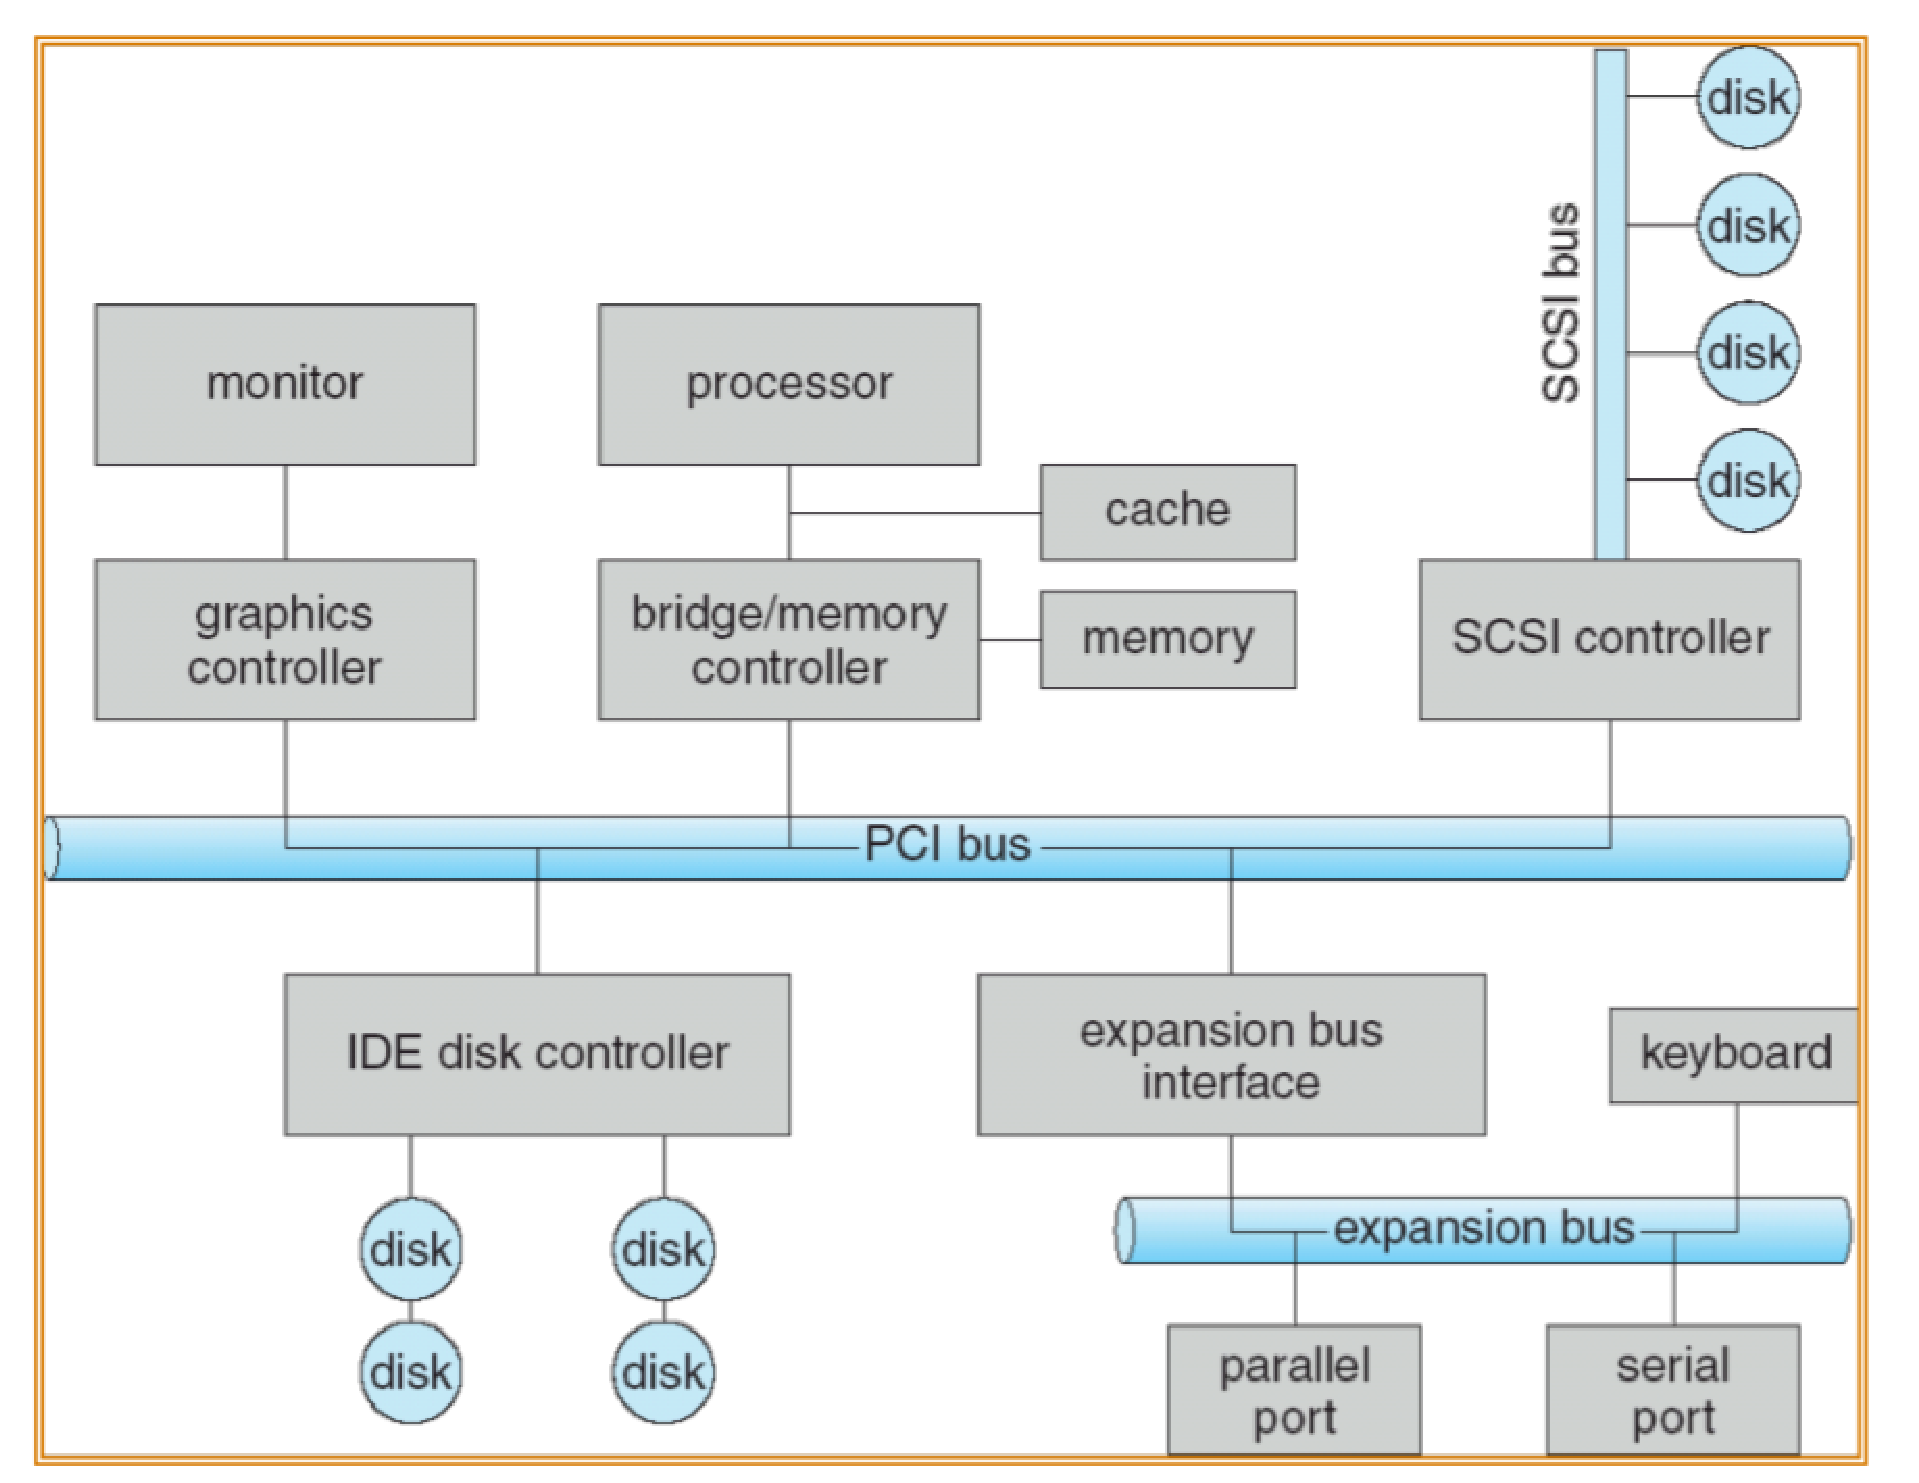
\includegraphics[height=4cm,
  angle=0]{./images/IO_architecture.eps}}
  \caption{(A) I/O architecture on motherboard; (B) I/O architecture for Linux
  kernel}
  \label{fig:IO_architecture}
\end{figure}

\subsection{architecture of Linux I/O system}

The Linux O/S kernel organizes into different I/O subsystems to handle the
communication with these devices as given in Fig.\ref{fig:IO_architecture}(B).

For an I/O request from the user-space app, it is sent to the Linux kernel's I/O
sybstem and then goes through multiple steps as given in
Fig.\ref{fig:Life-cycle-IO-request}.

\begin{figure}[hbt]
  \centerline{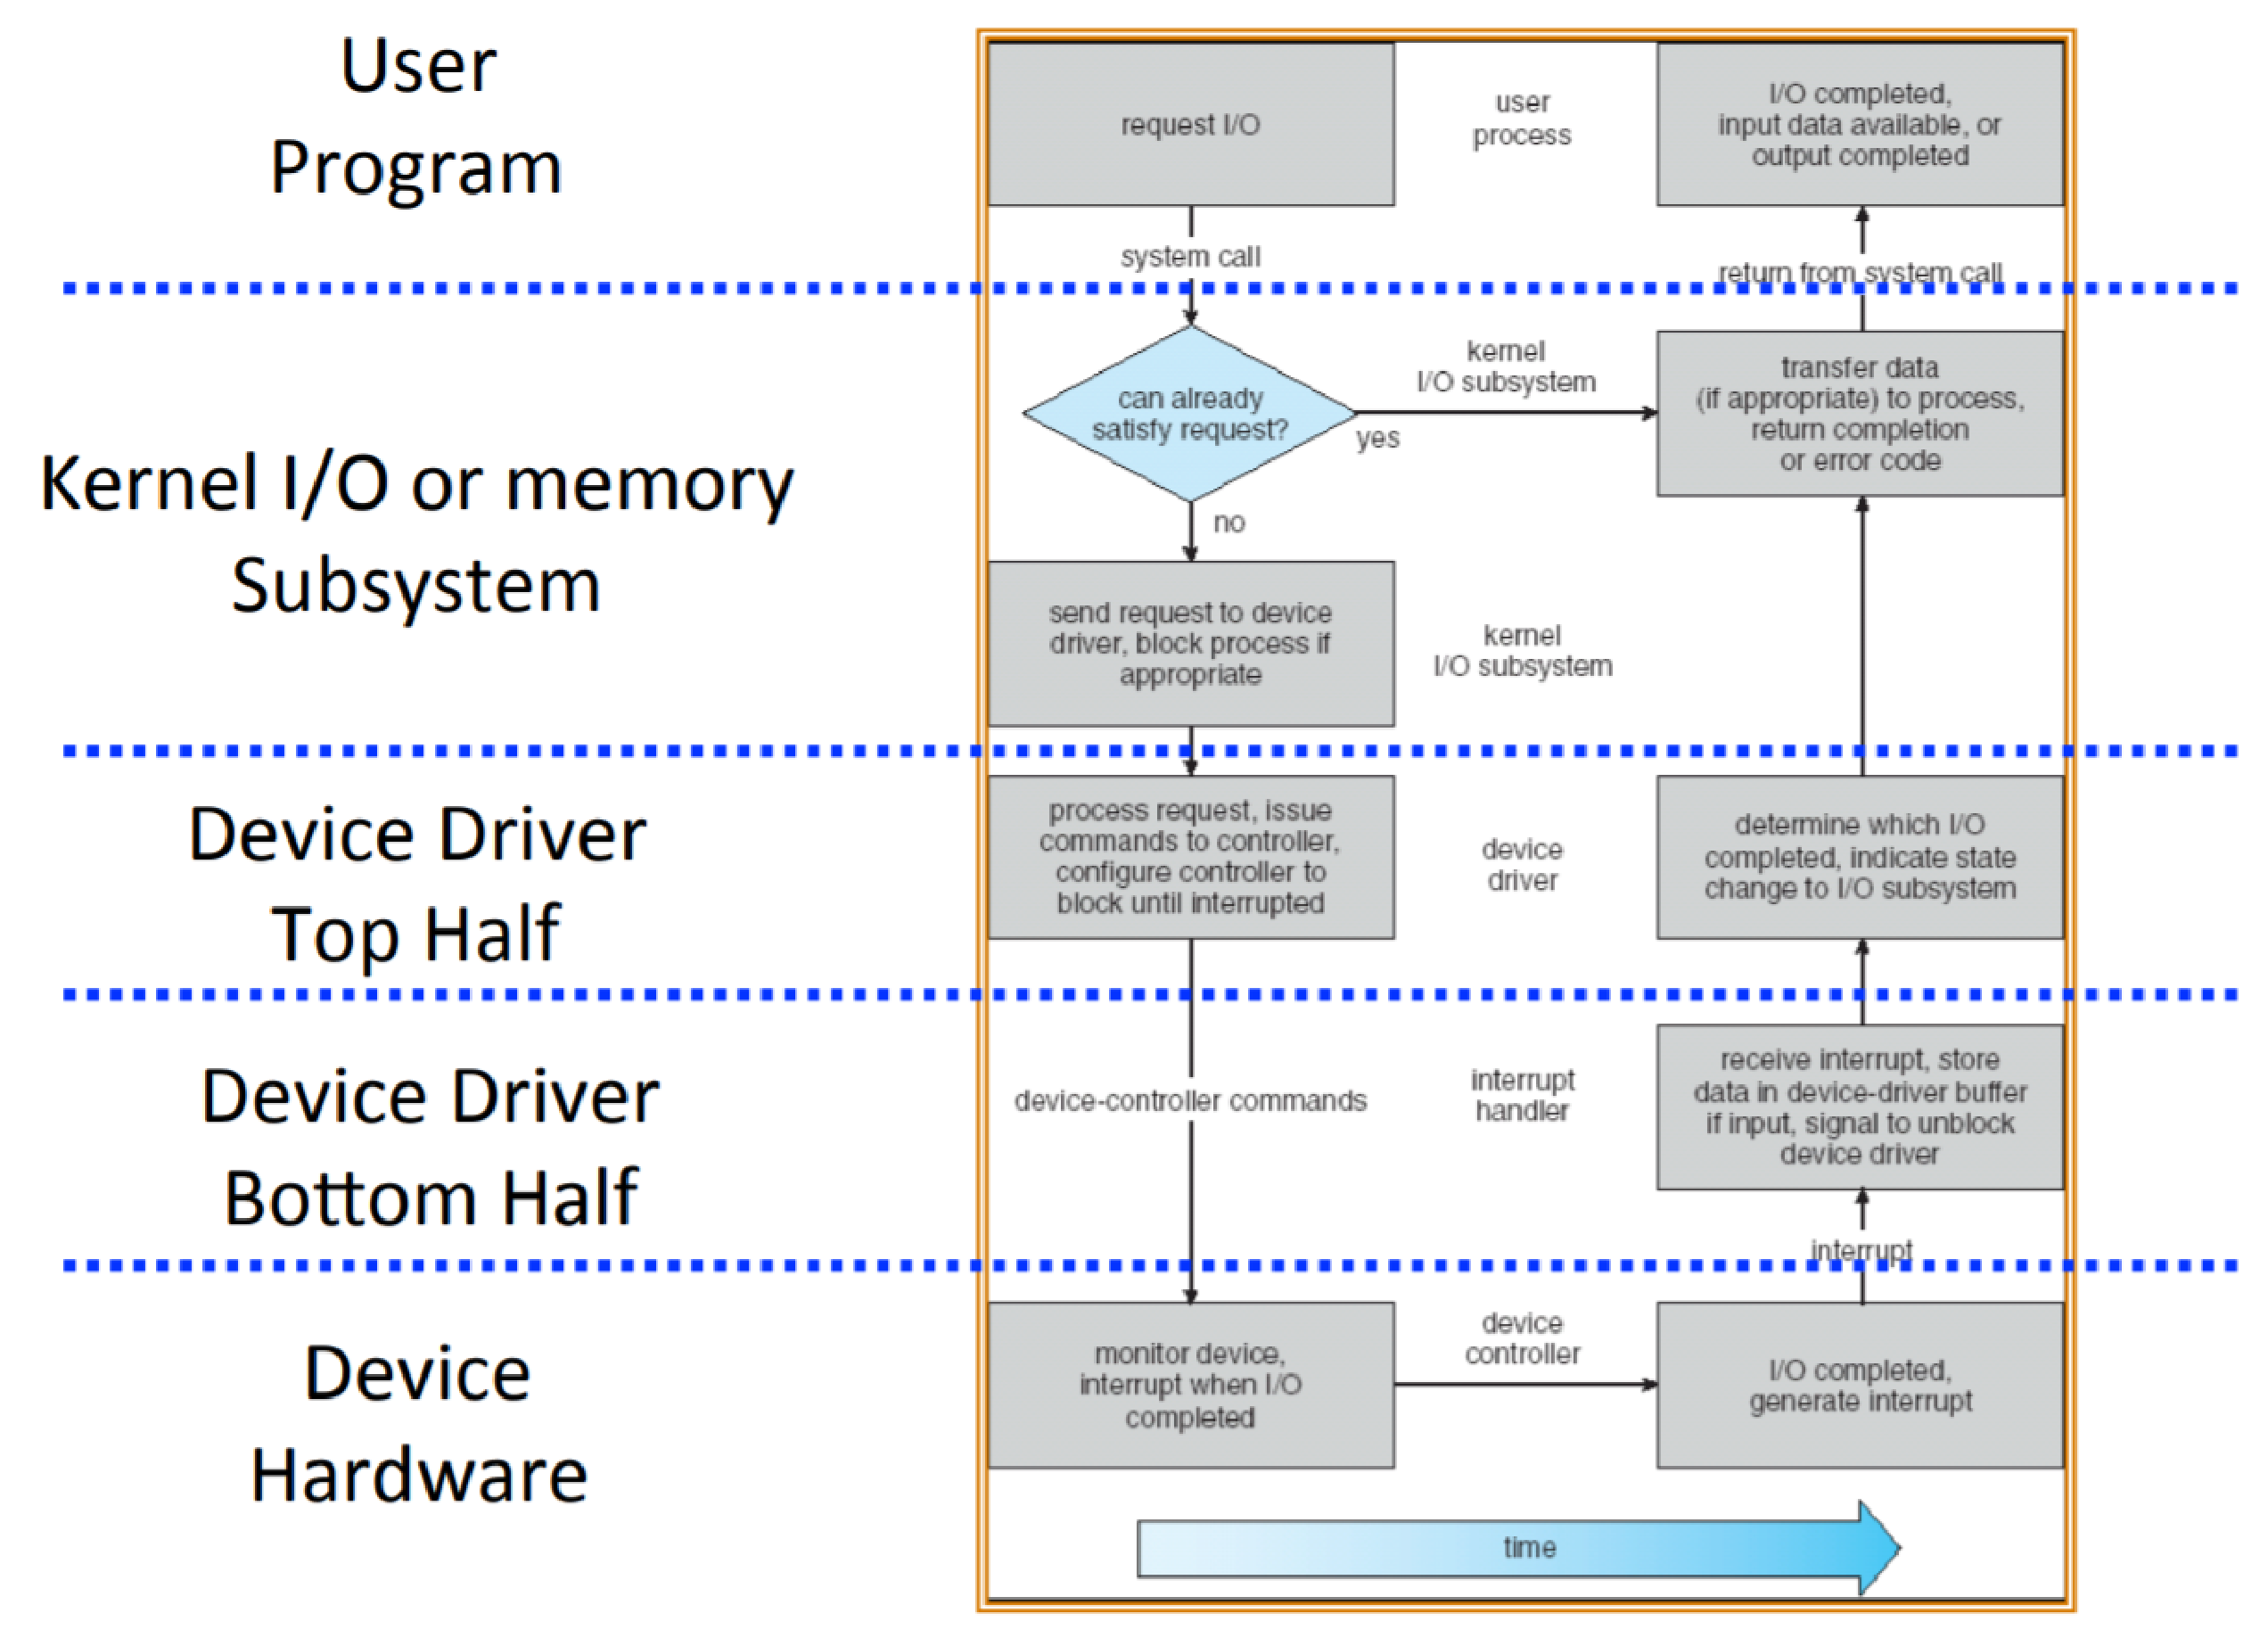
\includegraphics[height=4cm,
  angle=0]{./images/Life-cycle-IO-request.eps}}
  \caption{Life cycle of an I/O request}
  \label{fig:Life-cycle-IO-request}
\end{figure}

\subsection{DMA (direct-memory-access)}
\label{sec:DMA}
\label{sec:direct-memory-access}

When CPU issues a read/write statement, it goes through Linux kernel's I/O
substem which manages all I/O request. However, some times, you want full
control, e.g. direct read/write to the data on the device. This can be done
using {\bf DMA controller}, Fig.\ref{fig:DMA}.

\begin{figure}[hbt]
  \centerline{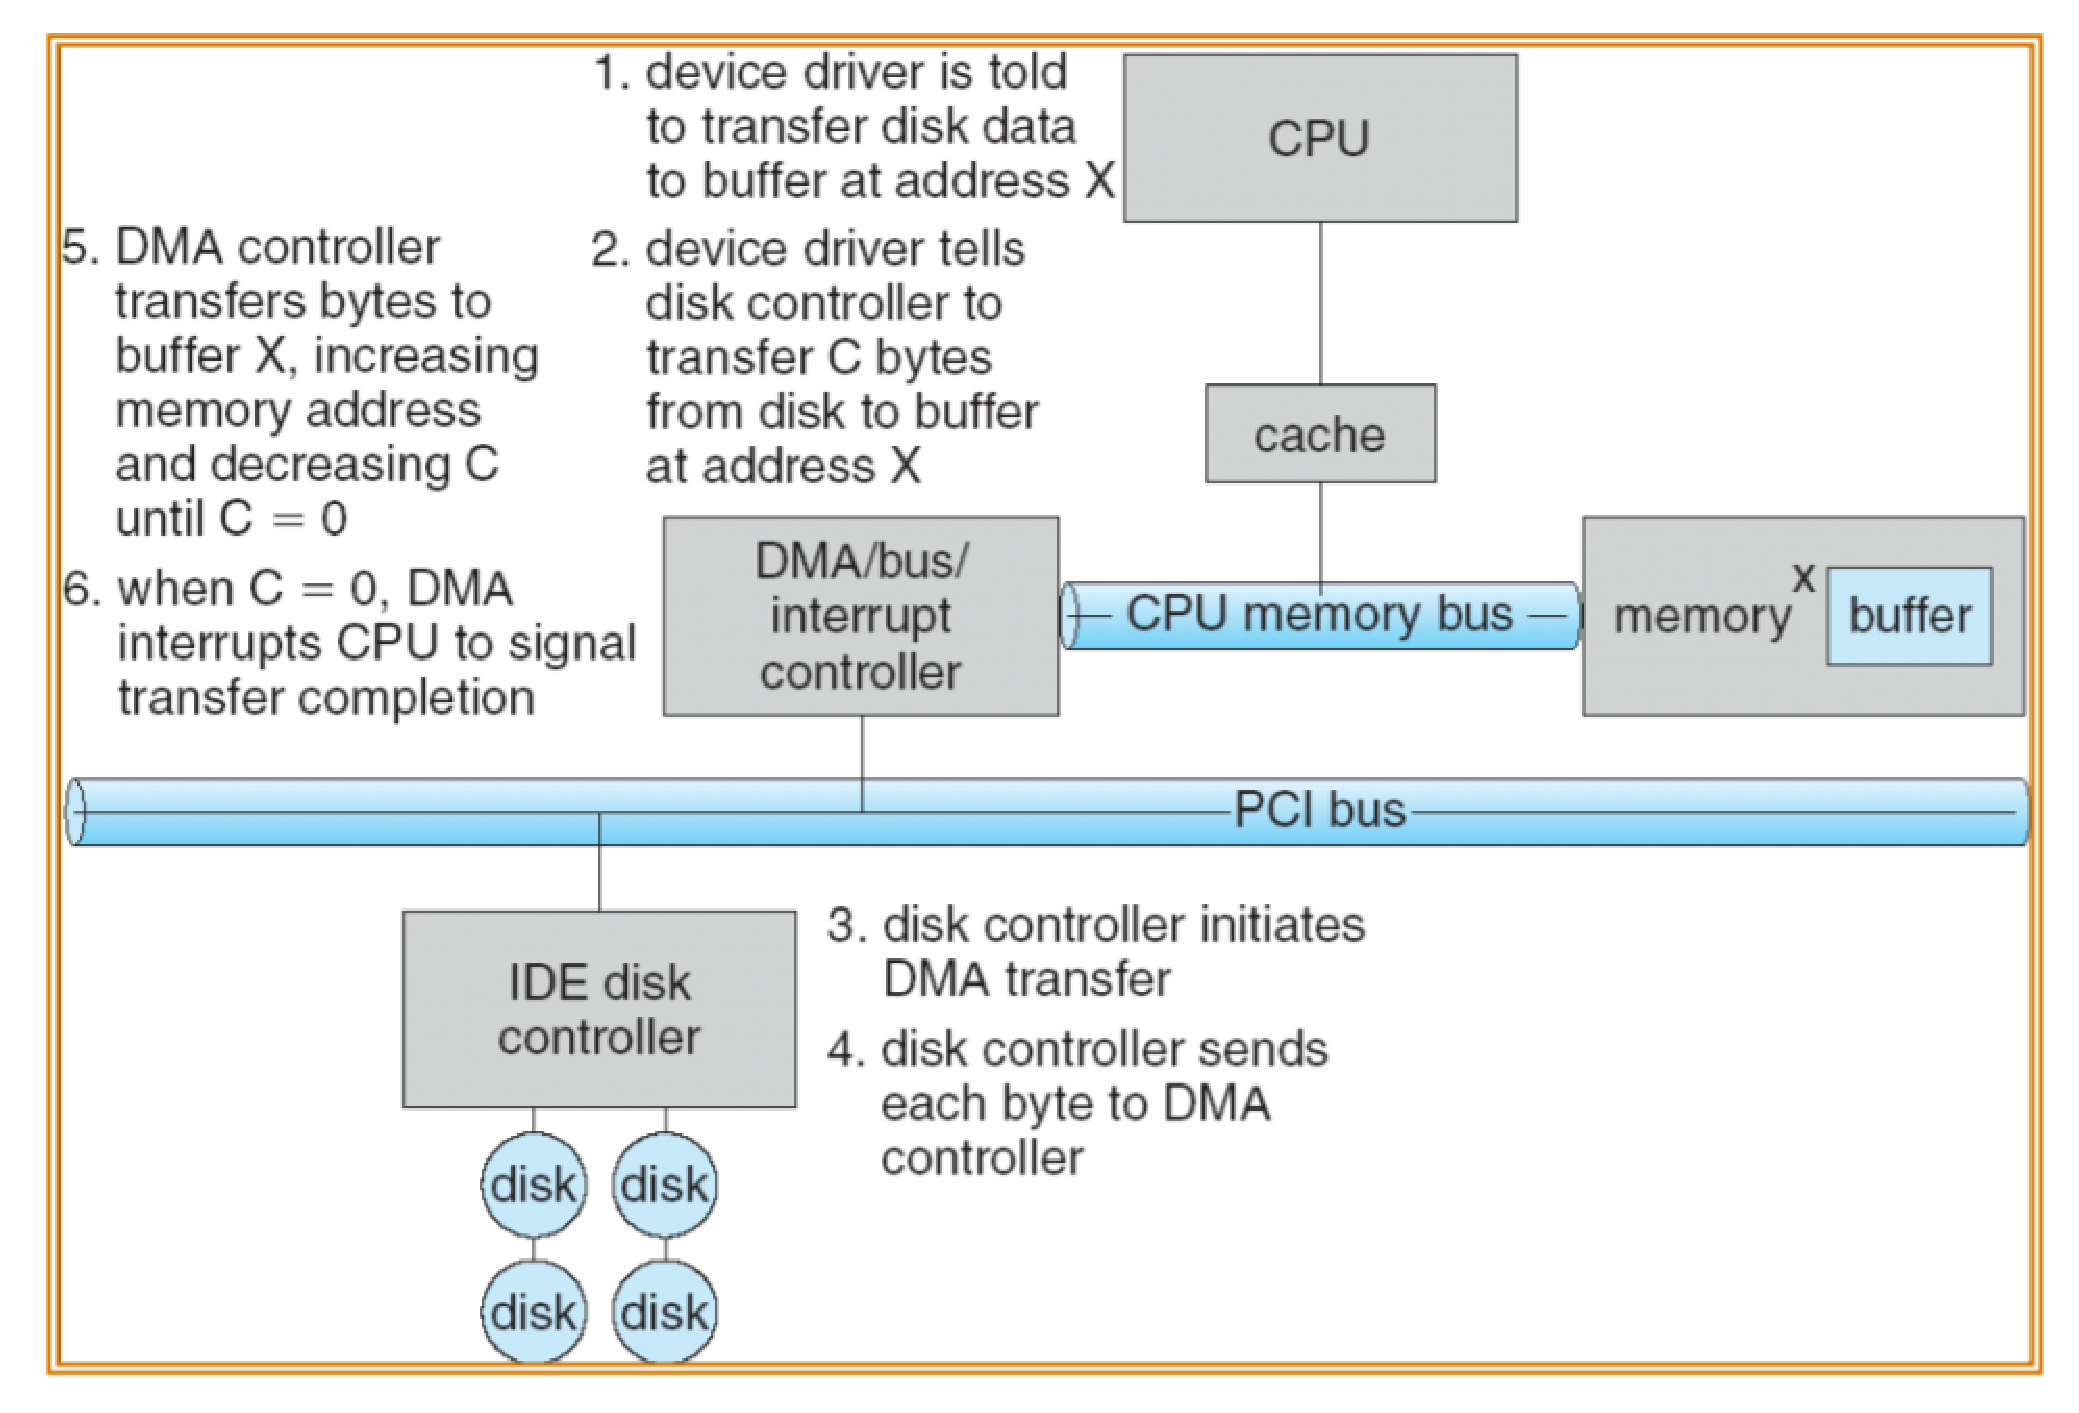
\includegraphics[height=4cm,
  angle=0]{./images/DMA.eps}}
  \caption{Direct-memory-access (DMA)}
  \label{fig:DMA}
\end{figure}



\section{Writing a device driver}

\subsection{Writing a simple 'char' driver}

We learn how to write a real device-independent driver: scull (Simple Character
Utility for Loading Localities). This driver acts on a memory area as thought it
were a device \footnote{\url{http://www.makelinux.net/ldd3/chp-3\#chp-3}}. 

A device can be accessed by name in \verb!/dev! folder. When we list the
content of this folder, a char device is identified by a 'c' in the first column
of the output of
\begin{verbatim}
ls -l
\end{verbatim}
A block device is identified by the 'b'.
\begin{verbatim}
bash-4.1$ ls -l
total 4
crw-rw-rw-  1 Tuan None  13, 254 Nov 30  2006 clipboard
crw-rw-rw-  1 Tuan None   5, 255 Feb  2 13:32 conin
crw-rw-rw-  1 Tuan None   5, 254 Feb  2 13:32 conout
crw-rw-rw-  1 Tuan None   5,   1 Feb  2 13:32 console
crw-rw-rw-  1 Tuan None  14,   3 Feb  2 13:32 dsp
lrwxrwxrwx  1 Tuan None       13 Sep  9  2011 fd -> /proc/self/fd
crw-rw-rw-  1 Tuan None   1,   7 Feb  2 13:32 full
crw-------  1 Tuan None   1,  11 Feb  2 13:32 kmsg
drwxrwxrwt+ 1 Tuan None        0 Sep  9  2011 mqueue
\end{verbatim} 
After 'None', the first number refer to the major number (which is the {\it
driver} associated with the device), and the second one is the minor number
(which is used by the kernel to know exactly which device it is referring to).
Major Linux kernels allow multiple drivers to share the same major number (so
it needs the minor number).

In the Linux kernel, the type \verb!dev_t! (\verb!/linux/types.h!) is used to
hold the device numbers (major and minor). In Linux 2.6.x, \verb!dev_t! is a
32-bit integer, with the first 12-bit for major number, and next 20-bit for
minor.



\section{Supercomputer - BlueGene IBM}
\label{sec:kernel_IBM_BlueGene}

Depending on the purpose of the node, 
\begin{enumerate}
  \item I/O node: Each node of the IBM BlueGene
supercomputer runs INK (I/O Node Kernel).
  \item Compute node: Each node runs CNK (Compute Node Kernel), a lightweight
  kernel that support a single application to run for a single user on that
  node. To maximize the performance, the kernel is small with physical memory is
  statistically mappedcd
\end{enumerate}
INK is a Linux-derivative

\section{Version control for Linux kernel}

Before 2002, there is no version control software being used for Linux kernel
development. From 2002, a commercial software name BitKeeper was used. Due to
coppyright issue, from 2005, Linus Torvalds and others developed {\bf Git} and
switched to using Git.



\section{time.h}
\label{sec:time.h}

\begin{verbatim}
struct timeval ---> define in /usr/include/bit/time.h
struct timespec --> define in /usr/include/time.h
\end{verbatim}
NOTE: \verb!struct timeval! has a BSD legacy whereas \verb!struct timespec! is
POSIX. So, make the decision based on the APIs you intend to use, rather than on
the structures themselves.
\textcolor{red}{Since POSIX.1-2008+TC1 some functions that use} 
\verb!struct timeval! are marked as obsolescent. \verb!struct timespec! is also part of the ISO C standard since C11.
\url{http://stackoverflow.com/questions/31275131/c-timeval-vs-timespec}
\url{http://stackoverflow.com/questions/20759750/resolving-redefinition-of-timespec-in-time-h}

There are API [in]compatibility:
\begin{itemize} 
  \item  POSIX-y calls like pselect() and \verb!clock_gettime()! use 
  \verb!struct timespec!
  
NOTE: Mac OS X does not support \verb!clock_gettime()!.
\verb!clock_gettime()! is not standard C99, nor is \verb!CLOCK_REALTIME!. But
they are POSIX (SUSv2, POSIX.1-2001).

  \item Various filesystem calls like utimes(), 
  and some assorted Linux calls like gettimeofday() and select(), use 
  \verb!struct timeval!

\verb!struct timeval! also has some comparison functions on Linux, BSD and Mac
OS X, e.g. timercmp(), timersub().

  \item
\end{itemize}



\begin{verbatim}
* POSIX.1b structure for a time value.  This is like a `struct timeval' but
   has nanoseconds instead of microseconds.  */
struct timespec
  {
    __time_t tv_sec;        /* Seconds.  */
    __syscall_slong_t tv_nsec;  /* Nanoseconds.  */
  };

#/usr/include/time.h  # which defines
  struct timespec
{
    __time_t tv_sec;            /* Seconds.  */
    long int tv_nsec;           /* Nanoseconds.  */
};
  
/usr/include/linux/time.h   # for Linux kernel 2.6.31.13
  struct timespec {
    __kernel_time_t tv_sec;                 /* seconds */
    long            tv_nsec;                /* nanoseconds */
}; 



/usr/include/time.h  # which defines
#ifndef _STRUCT_TIMESPEC
#define _STRUCT_TIMESPEC
struct timespec {
        time_t  tv_sec;         /* seconds */
        long    tv_nsec;        /* nanoseconds */
};
#endif /* _STRUCT_TIMESPEC */


/* A time value that is accurate to the nearest
   microsecond but also has a range of years.  */
struct timeval
  {
    __time_t tv_sec;        /* Seconds.  */
    __suseconds_t tv_usec;  /* Microseconds.  */
  }; 

/* some other they don't have '__' prefix */  
/* Timer ID returned by `timer_create'.  */
typedef __timer_t timer_t;
struct timeval {
        time_t          tv_sec;         /* seconds */
        suseconds_t     tv_usec;        /* microseconds */
};  

/* for kernel module since 2.6.31.3: some other use '__kernel_' prefix */
struct timeval {
         __kernel_time_t         tv_sec;         /* seconds */
         __kernel_suseconds_t    tv_usec;        /* microseconds */
};

\end{verbatim}

with  both \verb!__syscall_slong_t! and \verb!__suseconds_t! defined as a "long
 word". However, there is no consistent definition of \verb!time_t!.


\begin{verbatim}
The time_t datatype is a data type in the ISO C library defined for storing
system time values. Such values are returned from the standard time() library
function. This type is a typedef defined in the standard header. ISO C defines
time_t as an arithmetic type, but does not specify any particular type, range,
resolution, or encoding for it. Also unspecified are the meanings of arithmetic
operations applied to time values.

Unix and POSIX-compliant systems implement the time_t type as a signed integer
(typically 32 or 64 bits wide) which represents the number of seconds since the
start of the Unix epoch: midnight UTC of January 1, 1970 (not counting leap
seconds). Some systems correctly handle negative time values, while others do
not. Systems using a 32-bit time_t type are susceptible to the Year 2038
problem. 
\end{verbatim}
 To know the exact definition of \verb!__time_t! on your compiler chain, create
 a file \verb!test.c! with the content
\begin{verbatim}
#include <time.h>

int main(int argc, char** argv)
{
        time_t test;
        return 0;
}
\end{verbatim}
and run
\begin{verbatim}
gcc -E test.c | grep '__time_t'
\end{verbatim}
and the output is
\begin{verbatim}
__extension__ typedef long int __time_t;
typedef __time_t time_t;

\end{verbatim}
Typically, the definition is in \verb!include/bits/type.h!
\begin{verbatim}
#include <bits/typesizes.h>     /* Defines __*_T_TYPE macros.  */
 __STD_TYPE __TIME_T_TYPE __time_t;      /* Seconds since the Epoch.  */
\end{verbatim}
and check \verb!<bits/typesizes.h>! for the exact size.

\url{http://stackoverflow.com/questions/471248/what-is-ultimately-a-time-t-typedef-to}
% There are two files, which has the same definition of 
% \verb!struct timespec!
% \begin{verbatim}
% 
% \end{verbatim} 
% until Linux 2.6.31.13


The Year2038 problem: the time-elapsed since EPOCH time if stored in 32-bit will
be overflow when it reaches year 2038. This is no problem, if the time-elapsed
is stored into the string, and read back
\begin{verbatim}
FILE *stream = [stream file pointer that you've opened correctly];
fprintf (stream, "%d\n", (int)time_t);
\end{verbatim}
then read back the same way (with fscan, fread). However, if you save the data
in numeric form, it will be wrong.

Effor to redefine the datetime data structure using 64-bit
\url{https://lwn.net/Articles/644834/}
In LibC, 
\begin{verbatim}
# asm_i386/posix_types.h
typedef long long __kernel_time_t;
\end{verbatim}
\url{http://linuxfinances.info/info/unix2038.html}
\url{http://www.cs.fsu.edu/~baker/devices/lxr/http/source/linux/include/linux/time.h}


If for some reason there is a conflict, one way is to write a barrier check code 
\begin{verbatim}
#ifndef _STRUCT_TIMESPEC
#define _STRUCT_TIMESPEC
struct timespec {
        time_t  tv_sec;         /* seconds */
        long    tv_nsec;        /* nanoseconds */
};
#endif /* _STRUCT_TIMESPEC */
\end{verbatim}
or (2) just rename
\begin{verbatim}
#include <time.h>
#define timespec linux_timespec
#include <linux/time.h>
#undef timespec
\end{verbatim}
and assert at compile time that both have the same layout
\begin{verbatim}
typedef int assert_same_size[sizeof(struct linux_timespec) == sizeof(timespec) ? 1 : -1];
typedef int assert_same_alignment[__alignof(struct linux_timespec) == __alignof(timespec) ? 1 : -1];
typedef int assert_same_tv_sec[offsetof(struct linux_timespec, tv_sec) == offsetof(struct timespec, tv_sec) ? 1 : -1];
typedef int assert_same_tv_nsec[offsetof(struct linux_timespec, tv_nsec) == offsetof(struct timespec, tv_nsec) ? 1 : -1];
\end{verbatim}

\subsection{CLOCK\_REALTIME}


If you get 
\begin{verbatim}
error: 'CLOCK_REALTIME' undeclared (first use in this function)
\end{verbatim}
to fix, compile the code with \verb!-std=gnu99!. If you want to use
\verb!std=c99!, you may get the above error as \verb!CLOCK_REALTIME! is not part
of C99, so to resolve, try adding
\begin{verbatim}
   # GCC
-D_POSIX_C_SOURCE=199309
   # G++
-D_GNU_SOURCE=199309   
\end{verbatim} 
on the gcc command line, or in a header file 
\begin{verbatim}
#define _POSIX_C_SOURCE >= 199309L
 $ or
#define _POSIX_C_SOURCE=200112L 
\end{verbatim}
\textcolor{red}{before}
\verb!#include <time.h>! as this is a necessary feature test macro requirement.
\url{http://stackoverflow.com/questions/13069758/got-compile-error-when-use-clock-gettime-in-c99}
\url{https://groups.google.com/forum/#!topic/gnu.gcc.help/KkDn436ukEM}
%, might expose clock_gettime (per the clock_gettime 'man'  page). 


\section{if.h (interface)}
\label{sec:if.h}

\verb!IFNAMSIZ!
\begin{verbatim}
#define IFNAMSIZ 16
\end{verbatim}
This constant defines the maximum buffer size needed to hold an interface name,
including its terminating zero byte.

If you get the error
\begin{verbatim}
error: 'IFNAMSIZ' undeclared here (not in a function) 
\end{verbatim}
then make sure \verb!#include <linux/if.h>! is added to the file that uses
IFNAMSIZ.

\section{POSIX standard /pahz-icks/ vs. Single Unix Specification (SUS)}

\subsection{UNIX war - X/Open group vs OSF}
\label{sec:UNIX-war}

It was not easy to set the standard between UNIX vendors, i.e. UNIX wars in the
late 1980s and early 1990s.\footnote{\url{http://en.wikipedia.org/wiki/Unix_wars}} 
In 1984, a group of vendors formed {\bf X/Open standards group} (to create
compatible O/S). Then, AT\&T and Sun formed an alliance to develop System V. 
In the mid-1980s, the two most common UNIX are BSD (Berkeley) and System V
(AT\&T).

In response to the threat of 'merged UNIX system' by AT\&T and Sun, in 1988,
{\bf OSF} (Open Software Foundation) was created by a number of vendors (HP,
Apollo Computer, DEC, IBM, etc.).

To help standardize the system interface, i.e. system APIs, POSIX was created.
In 1988, POSIX standards become IEEE 1003 (ISO/IEC 9945) and IEEE charged a fee
to access. 


\subsection{-- XPG}
\label{sec:XPG}

To void the fee of using POSIX charged by IEEE, X/Open developed {\bf XPG}
(X/Open Portability Guides), in parallel with POSIX. 

\begin{mdframed}

The macros to determine code based on X/Open (XPG) is
\begin{verbatim}
__USE_XOPEN
__USE_XOPEN_EXTENDED
__USE_XOPEN2K
\end{verbatim}
\url{http://web.mit.edu/jhawk/mnt/spo/phone-project/include/stdlib.h}
\url{http://stackoverflow.com/questions/5378778/what-does-d-xopen-source-do-mean}

To add code 

\url{http://man7.org/linux/man-pages/man7/feature_test_macros.7.html}
\end{mdframed}

\textcolor{red}{\bf XPG} is wider than POSIX, i.e. cover more specifications.
\footnote{\url{https://en.wikipedia.org/wiki/X/Open}}
\begin{enumerate}
  \item XPG2 (XPG Issue 2), issued in 1987, added terminal-handling API,
  i.e. System V \verb!curses!. 

  \item XPG3 merged with X11 API in 1990. After 1990, XPG
incorporated POSIX and added more features. 

  \item XPG4, in 1992, mandated full compliance with 1989 ANSI C standard. 
  
  \item XPG4.2: the last version then turned into CAE4 {\it (Common Applications
  Environment Specification Issue 4)} (or Spec 1170 or X/Open Programming Guide
  4.2 (XPG 4.2)).
\end{enumerate}

\subsection{OpenGroup: X/Open + OSF}

In 1996, X/Open and OSF merged to form the Open Group. Open Group now certifies
UNIX trademark, and publish Single Unix Specification (SUS) technical standard -
Sect.\ref{sec:SUS} (the core of SUS are developed and maintained by Austin Group
- a joint effort between Open Group, IEEE, ISO JTC 1 SC 22 Linux study group).



% Also before becoming standard (i.e.
% approved by ISO), the revisions, developed by Austin Group, are called {\bf
% Single UNIX Specification}. 

\subsection{SUS (Single Unix Specification): replace XPG}
\label{sec:SUS}

In 1993, seventy-five UNIX vendors declared supporting X/Open to put an end to
UNIX war with the new standard {\it Single UNIX Specification} (SUS) which is
based on XPG4 standard (Sect.\ref{sec:XPG}). Spec 1170 (XPG4.2) then become the
first version of SUS, and X/Open acquired the right to UNIX trademark.

\textcolor{red}{SUS encompass POSIX and XSI, i.e. extends the POSIX standard and
is the official definition of APIs of a UNIX system}. XSI (X/Open Group)
specifies a number of traditional UNIX interfaces which are unlikely to be
applicable to a new operating system that is not 'a UNIX'. 
\begin{itemize}
  \item Most Linux O/S are POSIX-compliant, and 

  \item UNIX O/S must be SUS-compliant. 
\end{itemize}

\begin{enumerate}
\label{sec:SUS-v1}  
  \item SUS version 1: UNIX95 standard (Sect.\ref{sec:UNIX95})
  
\label{sec:SUS-v3}  
  \item SUS version 2 (released 1997): UNIX98 standard (Sect.\ref{sec:UNIX98})

SUS version 2 addded ISO C90 (ISO/IEC 9899:1990) support and multibyte character
set (ISO/IEC 9899:1990/Amendment 1:1995 (E)) to the System Interfaces
Specification (XSH).

Successive versions of SUS try to deprecate parts of the XSI option; thus, the
later versions of SUS are getting closer to POSIX, e.g.
SUS version 3 == POSIX:2001. A bigger umbrella of standards that covers POSIX,
SUS, etc. is called LSB (Sect.\ref{sec:LSB}).

\label{sec:SUS-v3}
  \item SUS version 3 (release 2002): UNIX03 standard (Sect.\ref{sec:UNIX03}) or
  aka IEEE Std 1003.1.

IMPORTANT: SUS version 3 (SUSv3) has more than 3700 pages, divided into 4 parts:
XBD (Base Definitions, Issue 6 - Sect.\ref{sec:XBD}), XCU (Shell and Utilities -
Issue 6 - Sect.\ref{sec:XCU}), XSH (System Interfaces and Headers, Issue 6 -
Sect.\ref{sec:XSH}), XRAT (Rationale - Sect.\ref{sec:XRAT}).


  \item {\bf 2004: POSIX:2004}  (minor update): (formally: IEEE Std 1003.1-2004,
  now with incorporating two technical corrigenda)
  
\label{sec:SUS-v4}
  \item SUS version 4: {\bf 2008: Single UNIX Specification version 4,
  POSIX:2008} - Sect.\ref{sec:UNIX-V7}
  
  They are Issue 7 of the four core components.
  
  
\end{enumerate}
\url{http://pubs.opengroup.org/onlinepubs/7908799/index.html} 



\subsection{-- XBD}
\label{sec:XBD}

\subsection{-- XCU}
\label{sec:XCU}

The POSIX shell is an extension fo the Bourne shell based on the early version
of Korn shell. 

User-level programs include: awk, echo, ed, vi, \ldots



\subsection{-- XSH}
\label{sec:XSH}

XSH issue 4 was developed in 1994, incorporatd the draft of multibyte support
extension (MSE) in C language for international character sets (\verb!wchar_t!).
XSH issue 5 added the final version of MSE.

SUS version 2:
Systems Interfaces and Headers (issue 5)
\url{http://pubs.opengroup.org/onlinepubs/7908799/xshix.html}


\subsection{-- XRAT}
\label{sec:XRAT}

\subsection{POSIX}
\label{sec:POSIX}

{\bf POSIX} = Portable Operating System Interface for uniX, the name first
suggested by Richard Stallman to IEEE (pronounced: {\it pahz-icks}, not poh-six)
to define the unified APIs, and command-line shells, to maintain the
compatibility between UNIX operating systems.
\textcolor{red}{What does POSIX contains?} - it depends on the POSIX version,
but essentially it contains a lot of things: threads, semaphores, file system
access API, etc.

\url{http://www.opengroup.org/austin/papers/posix_faq.html} POSIX was first
maintained by IEEE {\it per se}, with POSIX.1 means IEEE Std 1003.1-1988.
Nowadays, POSIX is maintained by Austin Group (see below).
The latest version of the POSIX.1 standard is IEEE Std 1003.1, 2013 Edition,
developed by the Austin Group.

With more information added at different versions, IEEE Std 1003.1-1988 is just
a family of IEEE standards IEEE Std 1003.$n$, and is part of ISO/IEC 9945.
To avoid confusion, the meaning of POSIX has been revised, i.e. POSIX refers to
this family of standards IEEE Std 1003.$n$ and POSIX.1 means IEEE Std
1003.1-1988.

Before 1997, it has versions with different names:
POSIX.1 (IEEE Std 1003.1-1988), POSIX.1b (POSIX 1003.1-1993, real-time
extension), POSIX.1c (IEEE Std 1003.1c-1995, thread-extension), POSIX.2 (IEEE
Std 1003.2-1992, shell and utilities). Posix 1003.1e / 1003.2c  are abandoned
\url{http://users.suse.com/~agruen/acl/posix/posix.html}.


% In 2001, Open Group declared Single UNIX Specification version
% 3.

After 1997, all the names POSIX.1x are changed, with Austin Group began to
develop the combined standard (SUS version 3 and POSIX:2001)
\begin{itemize}
  \item POSIX.1-2001 (IEEE Std 1003.1-2001): SUS version 3. This is the core of
  UNIX 03 brand. \url{http://www.unix.org/version3/}
  
  \item POSIX.1-2004 (IEEE Std 1003.1-2004): two minor updates
  \item POSIX.1-2008 (IEEE Std 1003.1-2008): SUS version 4 
\end{itemize}

\begin{verbatim}
Beginning in 1998, a joint working group known as the Austin Group began to
develop the combined standard that would be known as the Single UNIX
Specification Version 3 and as POSIX:2001 (formally: IEEE Std 1003.1-2001). It
was released on January 30, 2002  
\end{verbatim}
and
\begin{verbatim}
In December 2008, the Austin Group published a new major revision, known as
POSIX:2008 (formally: IEEE Std 1003.1-2008). This is the core of the Single UNIX
Specification, Version 4 
\end{verbatim}  


\subsection{POSIX conformance vs. POSIX compliance}

Real-time embeded developers look into POSIX conformance.

POSIX compliance means the product provide only partial POSIX support. 
For Windows, only Windows Enterprise and Windows Ultimate editions are
POSIX-compliance.
\url{http://www.lynx.com/industry-solutions/industry-standards/posix/} 

\section{LSB (Linux Standard Base)}
\label{sec:LSB}

While SUS (Single UNIX Specification) is designed for UNIX O/S and POSIX is
designed for most UNIX-like O/S; LSB (Linux Standard Base) is the joint
standard (based on POSIX specification - Sect.\ref{sec:POSIX}) to promote the
compatibility between different Linux distributions (not UNIX systems).

\textcolor{blue}{LSB is not a single standard, but a set of standards}, and
POSIX is a part of LSB. Having LSB is important as nowadays, there are more
than 500 different Linux-based distros. From LSB 3.1, it's registered as an ISO
standard. To identify the conflict between LSB 3.1 and POSIX, ISO/IEC TR
24715:2006 was developed.

LSB is designed to be backward compatibility, i.e. binary-compatible and stable
ABI (Sect.\ref{sec:ABI}) for independent software vendors. It means that the
newer version always contain the older version, i.e. the interfaces are always
added, but not removed. There is always enough time for unused features, i.e.
interface deprecations, before it is completely removed from the standard.

LSB make sure compatibility at command-line levels and binary form. It includes
many other standards. NOTE: Somes are being adopted in UNIX systems as well.
\url{http://www.linux.org/threads/linux-standard-base-lsb.5113/}
\begin{enumerate}
  \item ISO C-language
  
  \item Itanium C++ ABI (ABI is the interface between software and the O/S -
  Sect.\ref{sec:ABI})
  
  \item Large File Support 
  
  \item POSIX : portable operating system interface (a family of standard
  specified by IEEE, i.e. EEE Std 1003.1-2008) to clarify and make uniform APIs.
  It covers 3 parts: Base definitions, System interfaces and headers,
  and Commands \& Utilities. 
  
Initially, UNIX systems follow POSIX standards, while POSIX can be implemented
on any O/Ss. Open Groups who control UNIX-trademark then created a standard 
only for UNIX and is based on POSIX and call it SUS (Sect.\ref{sec:POSIX}). Now,
the two standards (POSIX and SUS) are developed jointly at The Austin Group.

POSIX:2008 = IEEE Std. 1003.1-2008 = SUSv4 = The Open Group Specification Issue
7.\footnote{\url{http://unix.stackexchange.com/questions/14368/difference-between-posix-single-unix-specification-and-open-group-base-specifi}}
  
  \item SUS (Single Unix specifications) : a collection of standards with which
  any UNIX systems must comply, i.e. those comply with SUS belong to UNIX
  systems (Sect.\ref{sec:UNIX_standards}. 
  
  Examples of UNIX systems are HP-Unix and Mac OS X. Since Mac OS X 10.5+, it
  complies with POSIX 1003.1. Those that do not comply all Unix specifications
  are called Unix-like systems, e.g. Linux and *BSD.

  
  \item SVID (System V Interface Definition) : cover C-libraries, system calls,
  software and hardware management.
  
  \item System V ABI:
  
  \item X/Open curses : a standard for text-based user interfaces \verb!ncurses!
  - Sect.\ref{sec:ncurses}
  
  \item DWARF Debugging Information Format : the format being used by debuggers
  and compilers for reporting bugs.
  
  \item IEC 60559/IEEE 754 Floating Point
  
  \item ISO/IEC TR14652 - Character format specification
  
  \item ITU-T V.42 - Error correction standard
  
  \item Li18nux Globalization Specification (L18n) - Specifications that aid in
  the internationalization of Linux
  
  \item Linux Allocated Device Registry - Each type of /dev/ file has a special
  number. This registry is the officially set numbers.
  
  \item Mozilla's NSS SSL Reference : for Network Security Services and Secure
  Socket Layer \url{https://developer.mozilla.org/en-US/docs/NSS_reference}
  
  \item NSPR Reference - This is a reference for Netscape Portable Runtime (NSPR).

  \item RFC 1321 - The MD5 Message-Digest Algorithm

  \item RFC 1831/1832 - Remote Procedure Call Protocol Specification

  \item RFC 1833 - Binding Protocols for ONC RPC

  \item RFC 1950 - ZLIB Compressed Data Format Specification

  \item RFC 1951 - DEFLATE Compressed Data Format Specification

  \item RFC 1952 - GZIP File Format Specification

  \item RFC 2440 - OpenPGP Message Format

  \item RFC 2821 - Simple Mail Transfer Protocol (SMTP)

  \item RFC 2822 - Internet Message Format

  \item RFC 791 - Internet Protocols

  \item RPM Package Format - The RPM installation package (yes, the same one
used on Fedora and RedHat) has a standard that it follows.
\end{enumerate}

LSB is composed of two parts: (1) a common part that describes the constant
interface across all hardware implementations, (2) specific part that describes
the specification that are specific to a particular CPU architecture. 

From LSB 2.0, LSB is modularized to (LSB-core, LSB-CXX, LSB-graphics, LSB-L18n),
which includes specifications for (1) filesystem hierarchy, (2) binary format,
(3) a number of commands and utilities, (4) printing module (e.g.
CUPS), etc. 

Since LSB 3.0, LSB is registered as ISO/IEC 23360 with 8 different parts
(Sect.\ref{sec:LSB_3.1}).
\begin{enumerate}
  \item LSB-core: the general basis of specification
  \item LSB-C++ : the specifications for libraries
  \item LSB-Desktop: the specifications for GTK, QT3/QT4, multimedia (e.g.
  ALSA), graphics and others
  \item LSB-Languages: specification for Python, Perl, GTK+
  \item LSB-Printing: the standardized CUPS library
  \item LSB-security: the security specifications
\end{enumerate}

\subsection{LSB-compliant O/S}
\label{sec:LSB-compliant-OSes}

\textcolor{red}{O/S accepting the same LSB will have binary-compatible, and a
stable ABI (Sect.\ref{sec:ABI})}. The software packages must be
delivered either in LSB-compliant installer or RPM-package manager format.
\textcolor{red}{However, LSB has been criticized for not taking inputs from big
projects like Debian.} Thus, to install RPM packages in Debian-based systems,
end-users need to use Debian's Alien program to transform them into native
package format to install (Sect.\ref{sec:alien}).

Ubuntu 11.10 and 12.04 use LSB 4.0.  Red Hat Enterprise Linux, Oracle Linux,
SuSE Linux Enterprise and Mandriva Enterprise Server are LSB-compliant distros,
with the same RPM-based package manager.

To get basic info about which LSB specifications your O/S complies with, run 
\begin{verbatim}
lsb_release -a
\end{verbatim}
Example output: (we may need to install \verb!sudo apt-get install lsb-core! if
you get \verb!No LSB modules are available.! message)
\begin{verbatim}
LSB Version:   core-2.0-amd64:core-2.0-noarch:core-3.0-amd64:core-3.0-noarch:
   core-3.1-amd64:core-3.1-noarch:core-3.2-amd64:core-3.2-noarch:
   core-4.0-amd64:core-4.0-noarch
Distributor ID: Ubuntu
Description:    Ubuntu 10.04.1 LTS
Release:        10.04
Codename:       lucid
\end{verbatim}
 
\url{http://www.linuxfoundation.org/collaborate/workgroups/lsb}

\url{https://wiki.linuxfoundation.org/en/LSB_Wiki}


\subsection{System initialization}
\label{sec:LSB_system-initialization}

It's Chapter 18 (VII) in LSB 1.0. It's Chapter 14 in LSB 2.0.1. It's Chapter 20
in LSB 3.1.

Since LSB 3.1, a system conforming to LSB should has the following directories
or symbolic links to directories
\begin{enumerate}
  \item /etc/cron.d, /etc/crond.hourly, /etc/cron.daily,
  /etc/cron.weekly, /etc/cron.monthly (LSB 3.1):  folders that contains shell
  scripts to be executed at a given time information
  
  \item /etc/init.d (LSB 3.1): folder contain the initialization scripts, i.e.
  scripts that automatically run at system bootup (See Sect.\ref{sec:LSB_3.1}
  to know how to write an initialization script)
  
  \item /etc/profile.d (LSB 3.1): the directory contains shell scripts (same
  name conventions like cron jobs, but with \verb!.sh! extension. Without this
  extension, the behavior is unspecified).
\end{enumerate}

A LSB-compliant script (shell scripts, Perl scripts, etc.) should 
\begin{enumerate}
  \item provide at least 5 options

\begin{verbatim}
/etc/init.d/my_script 
        start, stop, restart, force-reload, and status
\end{verbatim}
optioinal options: try-restart|reload

  \item return a proper exit code
  \item document run-time dependencies
\end{enumerate}
They should be scripts, not binary files, so that can be modified by local
administrators.

To log the message, it can use \verb!init.d! functions
\begin{verbatim}
log_success_msg
log_failure_msg
\end{verbatim}
This default set of functions can be checked in \verb!/lib/lsb/init-functions!. 

To write the script (e.g. /etc/init.d/postgresql), first the header
\url{http://www.thegeekstuff.com/2012/03/lsbinit-script/}
\begin{verbatim}
### BEGIN INIT INFO
# Provides:          my_daemon
# Required-Start:    postgresql networking
# Required-Stop:     postgresql networking
# Default-Start:     2 3 4 5
# Default-Stop:      0 1 6
# Short-Description: This is a test daemon
# Description:       This is a test daemon
#                    This provides example about how to
#                    write a Init script.
### END INIT INFO
\end{verbatim}
Example:
\begin{verbatim}
### BEGIN INIT INFO
# Provides:          sudo
# Required-Start:    $local_fs $remote_fs
# Required-Stop:
# X-Start-Before:    rmnologin
# Default-Start:     2 3 4 5
# Default-Stop:
# Short-Description: Provide limited super user privileges to specific users
# Description: Provide limited super user privileges to specific users.
### END INIT INFO
\end{verbatim}

\begin{mdframed}
NOTE: As the script file calls some binary files, to avoid the script fails
obscurely when the script file remains, but the package has been removed, we
should always use a test statement
\begin{verbatim}
test -f program-executed-later-in-file || exit 5
\end{verbatim}

NOTE: Be sure to use a proper exit code
\begin{verbatim}
0	program is running or service is OK
1	program is dead and /var/run pid file exists
2	program is dead and /var/lock lock file exists
3	program is not running
4	program or service status is unknown
5-99	reserved for future LSB use
100-149	reserved for distribution use
150-199	reserved for application use
200-254	reserved
\end{verbatim}
\end{mdframed}

Then the body (NOTE: change DAEMON,PIDFILE,NAME variables and the
header above to meet your own script)
\begin{verbatim}
# Using the lsb functions to perform the operations.
. /lib/lsb/init-functions
# Process name ( For display )
NAME=my-daemon
# Daemon name, where is the actual executable
DAEMON=/home/user1/my_daemon
# pid file for the daemon
PIDFILE=/var/run/my_daemon.pid

# If the daemon is not there, then exit.
test -x $DAEMON || exit 5

case $1 in
 start)
  # Checked the PID file exists and check the actual status of process
  if [ -e $PIDFILE ]; then
   status_of_proc -p $PIDFILE $DAEMON "$NAME process" && status="0" || status="$?"
   # If the status is SUCCESS then don't need to start again.
   if [ $status = "0" ]; then
    exit # Exit
   fi
  fi
  # Start the daemon.
  log_daemon_msg "Starting the process" "$NAME"
  # Start the daemon with the help of start-stop-daemon
  # Log the message appropriately
  if start-stop-daemon --start --quiet --oknodo --pidfile $PIDFILE --exec $DAEMON ; then
   log_end_msg 0
  else
   log_end_msg 1
  fi
  ;;
 stop)
  # Stop the daemon.
  if [ -e $PIDFILE ]; then
   status_of_proc -p $PIDFILE $DAEMON "Stoppping the $NAME process" && status="0" || status="$?"
   if [ "$status" = 0 ]; then
    start-stop-daemon --stop --quiet --oknodo --pidfile $PIDFILE
    /bin/rm -rf $PIDFILE
   fi
  else
   log_daemon_msg "$NAME process is not running"
   log_end_msg 0
  fi
  ;;
 restart)
  # Restart the daemon.
  $0 stop && sleep 2 && $0 start
  ;;
 status)
  # Check the status of the process.
  if [ -e $PIDFILE ]; then
   status_of_proc -p $PIDFILE $DAEMON "$NAME process" && exit 0 || exit $?
  else
   log_daemon_msg "$NAME Process is not running"
   log_end_msg 0
  fi
  ;;
 reload)
  # Reload the process. Basically sending some signal to a daemon to reload
  # it configurations.
  if [ -e $PIDFILE ]; then
   start-stop-daemon --stop --signal USR1 --quiet --pidfile $PIDFILE --name $NAME
   log_success_msg "$NAME process reloaded successfully"
  else
   log_failure_msg "$PIDFILE does not exists"
  fi
  ;;
 *)
  # For invalid arguments, print the usage message.
  echo "Usage: $0 {start|stop|restart|reload|status}"
  exit 2
  ;;
esac
\end{verbatim}

At the end, to make the script start or stop automatically, run
\begin{verbatim}
update-rc.d <script_filename> defaults
\end{verbatim}
which will add appropriate 'S' and 'K' entries to the given run-levels, after
checking the dependencies.

\url{https://refspecs.linuxfoundation.org/LSB_2.0.1/LSB-generic/LSB-generic/iniscrptact.html}

\subsection{LSB 1.x (2001)}

There are 4 minor versions: 1.0, 1.1, 1.2 (1.2.1) and 1.3.
\begin{enumerate}
  \item 1.0: The first version LSB 1.0 do NOT standardize any libraries for C++ due to the
immaturity of the C++ ABI for name mangling, exception handling, etc.

\url{https://refspecs.linuxfoundation.org/LSB_1.0.0/gLSB.html}

System initialization in LSB 1.0
\url{http://refspecs.linuxfoundation.org/LSB_1.0.0/gLSB.html}
 
   \item 1.1: add hardware support (IA-32)
   \item 1.2: add hardware support (PowerPC 32-bit, IA-64)
   \item 1.2.1: add hardware support (Itanium)
   \item 1.3: add hardware support (Enterprise System Architecture/390,
   z/Architecture)
\end{enumerate}


\subsubsection{LSB 1.1 (2002)}

LSB 1.1. was released in Jan, 2002. It add one new common part and one
processor specific specification for IA32 architecture.

\url{https://refspecs.linuxbase.org/LSB_1.1.0/}

\subsubsection{LSB 1.2}

LSB 1.2 (June 2002) add a common specification, and one processor specific
specification for IA32, IA64, and PPC32 architecture.

\url{https://refspecs.linuxbase.org/LSB_1.2.0/}

\url{https://refspecs.linuxbase.org/LSB_1.2.0/gLSB/book1.html}

\subsubsection{LSB 1.3 }

LSB 1.3 adds hardware specific support: Itanium

\subsection{LSB 2.x (2004)}

Since LSB 2.0, it is  modularized to 4 parts (LSB-core, LSB-CXX, LSB-graphics,
LSB-I18n), except the last part was not released. 

There are three minor versions:
\begin{enumerate}
  \item 2.0: add hardware support for PowerPC 64-bit, AMD64), and synchronize with SUS version 3
(Sect.\ref{sec:POSIX}).
  \item 2.0.1 : release ISO version of LSB 2.0 (no LSB-graphics)
  \item 2.1 : 
\end{enumerate}

Chapter 14 of LSB 2.0.1 specifies system initialization (LSB-core)
\footnote{\url{https://refspecs.linuxfoundation.org/LSB_2.0.1/LSB-generic/LSB-generic/sysinit.html}}

\subsection{LSB 3.x (2005)}
\label{sec:LSB_3.1}
\label{sec:LSB_3.x}

Since LSB 3.0, LSB is registered as an official ISO standard, with 8 parts..
\begin{enumerate}
  \item ISO/IEC 23360-1:2006 (part 1: generic specification)
  \item ISO/IEC 23360-2:2006 (part 2: specification for IA-32)
  \item ISO/IEC 23360-3:2006 (part 3: specification for IA-64)
  \item ISO/IEC 23360-4:2006 (part 4: specification for AMD64)
  \item ISO/IEC 23360-5:2006 (part 5: specification for PPC32)
  \item ISO/IEC 23360-6:2006 (part 6: specification for PPC64)
  \item ISO/IEC 23360-7:2006 (part 7: specification for S390)
  \item ISO/IEC 23360-8:2006 (part 8: speficiation for S390x)       
\end{enumerate}


There are 3 minor versions:
\begin{enumerate}
  \item 3.0 : use GNU C Library 2.3.4, C++ ABI is changed (used by gcc 3.4),
  core specification is updated based on ISO POSIX 2003, and Technical
  Corrigenda 1: 2005.
  
  \item 3.1: ISO/IEC 23360- year 2005
  \item 3.2: ISO/IEC 23360- year 2008
\end{enumerate}
LSB 3.1 and LSB 3.2 ares essentially based on glibc 2.3.4
(Sect.\ref{sec:glibc-2.x})

LSB 3.1 and POSIX conflict:
\url{https://personal.opengroup.org/~ajosey/tr20-08-2005.txt}


\subsection{-- LSB 3.1}
\label{sec:LSB_3.1}

Chapter 20 of LSB 3.1 specifies system initialization (LSB-core), i.e. the
scripts to be run at system booting up.
 \footnote{\url{http://refspecs.linuxfoundation.org/LSB_3.1.0/LSB-Core-generic/LSB-Core-generic/tocsysinit.html}}

At the current version of LSB, the folders (/etc/init.d, /etc/profile.d,
/etc/cron.[something]) needed to be known by the application. In the future, the
application can call \verb!lsbinstall! to handle the script setup, without
knowing the destination
folder.\footnote{\url{http://refspecs.linuxbase.org/LSB_3.1.1/LSB-Core-generic/LSB-Core-generic/etc.html}}

It is recommended to use script files, rather than binary files
(Sect.\ref{sec:LSB_system-initialization}. Init scripts are used to start/stop a
software/service. 
\begin{verbatim}
/etc/init.d/postgresql start|stop|restart|reload|force-reload|status
\end{verbatim}



\subsection{LSB 4.x (2008)}
\label{sec:LSB_4.x}

There are 2 minor versions:
\begin{enumerate}
  \item 4.0: use GNU C Library 2.4, binary compatible with LSB 3.x, easier to
  use SDK, support newer version of GTK and Cairo graphical libraries, simpler way to create LSB-compliant RPM packages, support Crypto API
  (via Network Security Services - NSS - library)
  
LSB 4.0 has some 'Trial Use': Java support, multimedia (ALSA), security (NSS),
desktop-miscellaneous (xdg-utils)
  
  \item 4.1:  new version of SDK, update Linux Application Checker and Linux
  Distribution Checkers, officially add (ALSA, NSS, xdg-utils) as submodules,
  update GTK+, Cairo, CUPS libraries; and add 3 new test suites
  
Remove: Java support (due to licensing issue)
\end{enumerate}
\url{http://www.linuxfoundation.org/collaborate/workgroups/lsb/lsb-41-release-notes}

LSB 4.1 currently support 7 architectures:  IA32, IA64, PPC32, PPC64, S390,
S390X, X86-64.

Ubuntu 11.10 and 12.04 follows LSB 4.0
\footnote{\url{https://launchpad.net/ubuntu/+source/lsb/}}


\url{http://www.ludism.org/~rwhe/LSB/pdf/LSB-Core-generic-try01.pdf}

\subsection{LSB 5.x}
\label{sec:LSB_5.x}

LSB 5.1, LSB standard supports seven architectures - IA32, IA64, PPC32, PPC64,
S390, S390X, and
X86-64.\footnote{\url{http://www.linux.org/threads/linux-standard-base-lsb.5113/}}

\section{ABI}
\label{sec:ABI}

If the Linux kernel is \verb!2.6.26-4-generic!. The 4 in this example is the
ABI.

ABI is something like a bridge between the kernel space and the other kernel
modules, i.e. we can extend kernel's function via these modules
(Sect.\ref{sec:kernel-modules}). ABI defines how data structures or
computational routines are accessed in machine code, which is a low-level,
hardware-dependent format; in contrast, an API defines this access in source
code, which is a relatively high-level, relatively hardware-independent, often
human-readable format.
\begin{enumerate}
  \item {\bf Linux ABI}:
  refers to a kernel-user space ABI, i.e. it defines exported functions are
  available directly from the kernel (vmlinux), so that a user-space
  applications/daemon can utilizes. 
  
  For the most part, users don't need to worry about the kernel ABI.
  If the user-space app is a kernel module, these functions allow the module to
  make use of subsystems in the kernel for memory management, device interfaces,
  filesystems (VFS), networking stacks, etc.
  It define the convention so that the the kernel executes compiled code.
  
  An ABI has to be defined for every instruction set, such as x86, x86-64, MIPS,
  ARMv7-A (32-Bit), ARMv8-A (64-Bit), etc. with the endianness, if both are supported.

For each build of the kernel, we get a list of exported functions. This is in a
file called Modules.symver in the build. We slightly prepare this file and
include it in the linux-image package as \verb!/boot/abi-KERNEL_VER!.
\begin{verbatim}
sdiff /boot/abi-4.4.0-112-generic /boot/abi-4.4.0-116-generic -s
\end{verbatim}
\url{https://wiki.ubuntu.com/KernelTeam/BuildSystem/ABI}

  \item 
\end{enumerate}

NOTE: There are two major notations for {\bf application binary interfaces}
(ABI): EABI (ARM), OABI (oarm/oabi). EABI = embedded application binary
interface.

OABI requires the CPU to have the hardware FPU (hard-float). There are two OABI
versions: oarm and oabi. EABI is designed to use software floating operation in
CPU without FPU, i.e.
softFPU.\footnote{\url{http://wiki.embeddedarm.com/wiki/EABI_vs_OABI}} Software
floating-point operations that use softFPU run 10x faster than OABI.
ARMv5TE use soft-floating so we use EABI.



\url{https://abi-laboratory.pro/tracker/timeline/linux/}

\section{UNIX brands}
\label{sec:UNIX_standards}

Most modern UNIX variants known today are licensed versions of one of the
original UNIX editions. Sun's Solaris, Hewlett-Packard's HP-UX, and IBM's AIX
are all flavors of UNIX that have their own unique elements and foundations.
For example, Sun's Solaris is UNIX, but incorporates many tools and extensions
designed to get the best out of Sun's own workstation and server hardware.

Different versions of UNIX standards are: UNIX93, UNIX95, UNIX98, UNIX03. 

\subsection{UNIX93}
\label{sec:UNIX93}

%UNIX93 is an Open Group specification, closed by X/Open in 1996. 

UNIX93 refers to systems before the creating Single UNIX Specification (SUS -
Sect.\ref{sec:SUS}]) that are compliant with UNIX-based specifications: XPG3,
XPG4, SVID, and AT\&T source code.

\subsection{UNIX95}
\label{sec:UNIX95}

UNIX95 refers to systems that are compliant to Single UNIX Specification version
1 (published 1994 - Sect.\ref{sec:SUS}). The systems need to satisfy
\begin{itemize}
  \item VSX4: core system calls and libraries
  \item VSC: commands and utilities test suite
  \item VSU: Single UNIX extension test suite
  \item VST: for transport interfaces
  \item Plum Hall or Perennial for C language
\end{itemize}

\subsection{UNIX98}
\label{sec:UNIX98}

UNIX98 refers to systems that are compliant to Single UNIX Specification version
2 (published 1997). UNIX98 adds more requirements to the UNIX95
(Sect.\ref{sec:UNIX95})
\begin{enumerate}
  \item VSX5 (large files,dynamic linking and MSE)
  \item VSTH (threads)
  \item and optionally VSRT (realtime)
\end{enumerate}

\subsection{UNIX03}
\label{sec:UNIX03}

UNIX03 refers to 2001: Single UNIX Specification version 3, POSIX:2001. This was
released on Jan-2002 with (Sect.\ref{sec:SUS}).

There are total 5 commercial UNIX-based O/S certified for UNIX03 standard
(Sect.\ref{sec:UNIX03}): AIX (Sect.\ref{sec:AIX}), macOS, Solaris, HP-UX and
Inspur K-UX. 

\subsection{ UNIX V7}
\label{sec:UNIX-V7}

The trademark {\bf UNIX V7} is used to indicate O/S compliant with SUS version 4
(Sect.\ref{sec:SUS})

\section{Compare O/S(es)}

\url{http://distrowatch.com/}

\subsection{Linux vs. UNIX}

UNIX was proprietary (non-free) operating systems (O/S) and is primarily based
on AT\&T code (System V). They primarily run on mid-range hardwares, e.g. IBM,
HP, Sun. You need to buy to use Unix O/S, e.g. HP-UX, Solaris, and Mac OS X.
Most commercial versions of Unix O/S are coded and optimized for a single, and
possibly many handful, hardware architecture. This makes Unix systems run very
fast on these processors.

The GNU project set to create an open-source clone of Unix, but didn't have a
kernel at first. Linus Torvalds wrote the first Linux kernel as a hoppy and
released under GPL license, which turned out to be the kernel being used in
Linux O/Ss nowadays. Linux O/S are Ubuntu, etc. Linux O/S are free and have more
applications than Unix.

\begin{mdframed}
The first operating system UNICS was created in 1969, which later renamed to
UNIX. \footnote{\url{https://code.google.com/p/unix-jun72/}} UNIX time-sharing
system went through from version 1 to version
7.\footnote{\url{http://gunkies.org/wiki/Unix_System_1}}

In 1973, UNIX (version 4) was written in C. This leads to the ancestral UNIX
diverged into a family of operating systems. The original motivation to
standardize UNIX was the rival between AT\&T and Berkeley.

4.x BSD Unix was developed from UNIX version 7 (1979). BSD 4.1 quickly become
popular, with the addition of \verb!vi! editor, job control facilities, and
improvement in signals, and TCP/IP networking.
\url{http://www.faqs.org/docs/artu/ch17s02.html}

System III is the basis of AT\&T (1981), which reworked UNIX version 7 terminal
interfaces into a cleaner, and more elegant form that is IMCOMPATIBLE with
Berkely BSD. System V Release 1 incorporated some BSD utilities, like \verb!vi!.

During the Unix wars, to bridge the gap between variants of UNIX O/S, UniForum
was created in Feb, 1983. UDS83 is the Uniform 1983 Draft Standard, which
describes core Unix systems (consisting a subset of System III kernel and
libraries + file-locking primitive). The second draft, UDS84, influenced the
APIs of System V Release 2 (SVr2). In 1985, AT\&T released SVID (System V
Interface Definition) - a formal description of SVr2 API, and incorporating
UDS84. We also have SVID2 and SVID3. SVID become the basis for POSIX standard
(Sect.\ref{sec:POSIX}).

In terms of file-sharing over networks, Sun's Network File System (NSF -
Sect.\ref{sec:NFS}) prevail AT\&T's Remote File System/Sharing (RFS), as Sun
make the code open-source. Similarly, the open-source X window system won Sun's
proprietary Networked Window System (NeWS).

After 1985, the main thrust of UNIX standardization passed to IEEE, with IEEE
1003 committee developed POSIX (Sect.\ref{sec:POSIX}).
\end{mdframed}


\url{http://www.ibm.com/developerworks/aix/library/au-unix-difflinux.html}

\subsection{Debian-based vs. RPM-based distros (Ubuntu vs. CentOS)}
\label{sec:CentOS}
\label{sec:Ubuntu}
\label{sec:Debian}


Ubuntu is Debiand-based distro; while CentOS is RPM-based distro (derived
from Redhat Enterprise Linux).
Both deliver the same performance. However, CentOS is more popular as web-host
server as it supports {\bf cPanel}. In term of package installation
\footnote{\url{http://en.wikipedia.org/wiki/List_of_software_package_management_systems}},
RPM (yum) is not much helpful in package-dependencies. Debian installer
(apt-get) automatically recognize dependencies and install them. Another thing
to consider  Ubuntu is hardware compatibility. Ubuntu is compatible with a 
broad range of hardware devices.


\url{http://www.pontikis.net/blog/five-reasons-to-use-debian-as-a-server}

In general, both Ubuntu and Debian do intend to be LSB-compliant
(Sect.\ref{sec:LSB}), which can be checked with \verb!lsb_release! command and
provide \verb!alien! program to enable installation of RPM-based packages
(Sect.\ref{sec:alien}).
However, they can make occasional divergences when necessary. The system layout
of Ubuntu
\url{http://askubuntu.com/questions/138547/how-to-understand-the-ubuntu-file-system-layout}

\subsection{-- Ubuntu 14.04}
\label{sec:Ubuntu-14.04-upgrade}

To Ubuntu 16.04 LTS
\begin{verbatim}
sudo do-release-upgrade
\end{verbatim}

If only kernel
\begin{verbatim}
//
//sudo apt-get install linux-image-generic-lts-xenial linux-generic-lts-xenial


apt-cache search linux-image

apt-get install linux-image-4.4.0-34-generic linux-image-extra-4.4.0-34-generic \ 
    linux-headers-4.4.0-34 linux-headers-4.4.0-34-generic
\end{verbatim}
\url{https://talk.plesk.com/threads/ubuntu-14-04-lts-hwe-eol-kernel-upgrade.338961/}

\subsection{Windows}

MinGW 4.8.0 (posix, dw2) provide a complete open-source programming tool in
Windows environment. An application written with MinGW can run in Windows,
without using any 3rd-party C-runtime DLLs; except it uses MSVCRT.DLL, the
Microsoft C runtime library. For multi-threaded applications, it needs to have a
freely distributed thread support DLL, provided by MinGW itself.

MinGW links to msvcrt.dll (on Windows Xp is at version 7.0.2600.5512 ).



\subsection{openSUSE}

\subsection{* 13.1}

Available: 2013-Nov-19

Kernel: 3.11 (first released in 2013-Sept)

GUI: KDE 4.11 or GNOME 3.10


\subsection{Wind River Linux}

\url{https://en.wikipedia.org/wiki/Wind_River_Systems#Wind_River_Linux}

In 2012, Wind River introduced a new version of Wind River Linux that was
developed from the Yocto Project.


\section{HPC Distros}

\subsection{UNIX System V}
\label{sec:UNIX_System-V}
\label{sec:System-V}

UNIX System V (SysV) is one of the first commercial version of UNIX O/S.
It was developed by AT\&T, with 4 major releases (1,2,3,4). UNIX System V
release 4, i.e. SVR4, is the most successful one. 

\subsection{MVS, z/OS (mainframe)}

MVS (Multiple Virtual Storage) is a mainframe computer operating system running
on System/370 (from 1970s), System/390 mainframe computer of IBM. Another
operating system running on System/390 is OS/390. The goal for OS/390 is
simplify the packaging and ordering elements needed for MVS operating system
[IBM ended OS/390-branded versions in 2004].  The MVS O/S undergone different
name changes (MVS/SP, MVS/XA, MVS/ESA, MVS/ESA OpenEdition) and the last one is
{\bf z/OS} from 2000. Different versions supported different UNIX
specifications, Fig.\ref{fig:IBM_operating-systems}. MVS/ESA is MVS Enterprise
System Architecture; and MVS/ESA OpenEdition is MVS/ESA version 4 release 3. Mid
1995, IBM change all MVS/ESA entities to OS/390 in late 1995 to run on
System/390 mainframe. MVS/ESA 5.2.2 (i.e. OS/390 release 1) incorporated XPG4
and 90\% the Single UNIX specifications defined in XPG4.2.

\begin{mdframed}
Branding is a concept that allows applications developed on one branded flavour
of UNIX to run unchanged on other branded UNIX systems. We have XPG4 Base brand,
XPG Base 95 brand, XPG4 UNIX brand.

\end{mdframed}

In 2000, IBM renamed System/390 to IBM eServer zSeries.  z/OS run on {\it IBM
System z}, a family of IBM mainframe computers (IBM System z9, IBM System z10,
IBM zEnterprise). 'z' means zero-downtime, i.e. the system was built with spare
components capable of hot failovers to ensure continuous operations.

31-bit Linux kernel is called 's390'; and 64-bit Linux kernel is called 's390x'.  
Until z/OS 1.5, the system can boot in either 31-bit or 64-bit mode. 
This was end in 2007. Nowadays, z/OS only supports 64-bit on z/Architecture
mainframes.

z/OS supports POSIX (1003.1, 1003.1a, 1003.1c, and 1003.2) with about 300
functions. UNIX System Services (USS), later renamed z/OS USS, is a required
component in z/OS. USS is XPG4 UNIX95 certified (Sect.\ref{sec:UNIX95}). 


\begin{figure}[hbt]
  \centerline{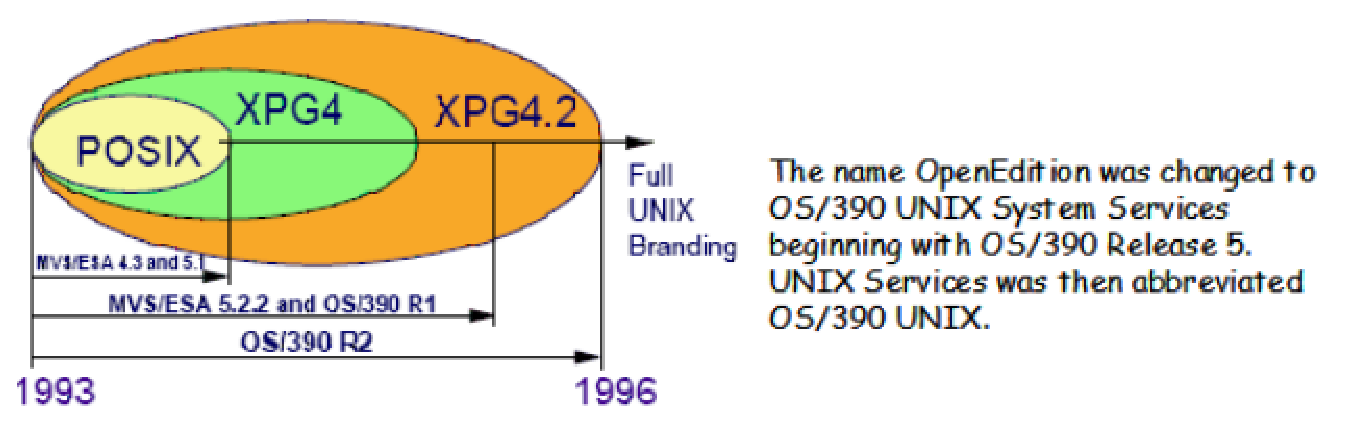
\includegraphics[height=3cm,
    angle=0]{./images/IBM_operating-systems.eps}}
  \caption{IBM Operating systems and supported UNIX specifications}
  \label{fig:IBM_operating-systems}
\end{figure}


\subsection{AIX}
\label{sec:AIX}

AIX is based on UNIX System V (Sect.\ref{sec:UNIX_System-V}) with
4.3BSD-compatible extensions.



\subsection{HP-UX}
\label{sec:HP-UX}

HP-UX is a Unix-OS derived from UNIX System V (Sect.\ref{sec:UNIX_System-V}).

To check MAC address on HP-UX machines
\begin{itemize}
  \item \verb!lanscan! command
  \item \verb!/opt/ignite/bin/print_manifest!
  \item \verb!lanadmin! and type ``lan display''
\end{itemize}


\subsection{Rocks}

Rocks is a distro built on top of CentOS with a lots of tools to make it easy to
automate building HPC clusters. 

\subsection{Manage Old Distribution of Ubuntu}

To fix problems related to 
\begin{verbatim}
apt-get update	
\end{verbatim}
we need to modify \verb!/etc/apt/sources.list!.

For distributions that are no-longer supported. You may not be able to install
new packages. To do so, we need to tell where it looks for  package
repositories. Open the file \verb!/etc/apt/sources.list! and change the
\verb!drb! and \verb!deb-src! lines from something like
\begin{verbatim}
http://us.archive.ubuntu.com/ubuntu
\end{verbatim}
to
\begin{verbatim}
http://old-releases.ubuntu.com/ubuntu/
\end{verbatim}
and from
\begin{verbatim}
http://security.ubuntu.com/ubuntu
\end{verbatim}
to 
\begin{verbatim}
http://old-releases.ubuntu.com/ubuntu
\end{verbatim}

If you get error
\begin{verbatim}
W: Failed to fetch
     http://ppa.launchpad.net/linuxdcpp-team/release/ubuntu/dists/
     lucid/main/binary-amd64/Packages.gz 404 Not Found
\end{verbatim}


References:
\begin{enumerate}
  \item
  \burl{http://serverfault.com/questions/286053/how-to-install-old-packages-for-ubuntu-9-04}
\end{enumerate}

\subsection{Ubuntu 11.10}

To disable the list of all users, we do
\begin{verbatim}
sudo -u gdm gconftool-2 --type boolean --set
/apps/gdm/simple-greeter/disable_user_list true
\end{verbatim}

\subsection{Ubuntu 12.04}

Ubuntu 12.04 use lightDM for X manager. For the list of configuration option, in
file /etc/lightdm/lightdm.conf, we see
\url{http://hmontoliu.blogspot.com/2011/10/disable-guest-sesson-in-ubuntu-1110.html}

To disable the Guest account, edit the file /etc/lightdm/lightdm.conf
\begin{verbatim}
allow-guest=false
\end{verbatim}

To disable the list of all users, we do
\begin{verbatim}
greeter-hide-users=true
\end{verbatim}


Finally, run
\begin{verbatim}
/etc/init.d/lightdm restart
\end{verbatim}

\subsection{IBM i}

IBM i (previously named OS/400 then i5/OS) is EBCDIC-based O/S runs on IBM Power
Systems and IBM PureSystems.

\subsection{RedHat 6}

\subsubsection{Display}

With nouveau:
\begin{enumerate}
  \item No support hibernate/suspend (system halt)
  \item No support \ldots 
\end{enumerate}

New laptop has Nvidia/Intel hybrid VGA, i.e. the system use Intel on battery and
use Nvidia on high performance graphical display. Nvidia Optimus technology
allows switching between them easily. However, it works well so far on Windows.
{\bf Bumblebee} is a free open-source effort to do that on Linux. 

Xorg: \url{http://www.x.org/archive/X11R6.8.2/doc/DESIGN2.html}


IMPORTANT: Do not use \verb!BusID   ``PCI:0:1:0''!, as it has to be in decimal
for Xorg.conf even though \verb!lspci! report HEX. So, we should either delete
or use the decimal value.

\url{http://www.x.org/wiki/FAQErrorMessages}

Check /var/log/Xorg.0.log, which tell which VGA device is being activated (the
one with \verb!*! ahead). 


On ThinkPad W520, with kernel 2.6.x, switching to 'Discrete Graphics' in Bios
booting halts. To resolve the problem, use in /boot/grub/grub.conf
\footnote{\url{https://bugzilla.redhat.com/show_bug.cgi?id=827164}}
\begin{verbatim}
pci=noacpi
  acpi=noirq
  noapic
  nolapic
  nox2apic
\end{verbatim}
However, this make the system disabled multicores, i.e. only a single core is
detected (check with \verb!cat /proc/cpuinfo!). A better solution is to goto
Bios, Security setting, Virtualization and disable two options: VT-d and Intel
Virtualization Technology. 

To test if nvidia-driver has been installed properly, run \verb!glxgear!
\begin{verbatim}
glxgear
\end{verbatim}
If you see the error
\begin{verbatim}
libGL error: failed to load driver: swart
\end{verbatim}
you may not have installed the 32-bit component of the driver. You just
need to reinstall the whole package.

\subsubsection{Media (MP4, MP3)}

We need to make sure
\begin{verbatim}
PackageKit-gstreamer-plugin.x86_64
gstreamer.x86_64
gstreamer-ffmpeg.x86_64 //need to download from rpbone
  ffmpeg-libs-0.10.12-1.5.el6.nux.x86_64.rpm
  libavutil51-1.0.6-57.el6.x86_64.rpm
  
  ffmpeg-libs-0.10.4-1.el6.nux.x86_64.rpm
  ffmpeg-libs-0.8.0-1.el6.nux.x86_64.rpm //dependencies
  libass-0.9.12-1.el6.nux.x86_64.rpm
  enca-1.13-1.el6.x86_64.rpm
  xvidcore-1.2.2-2.el6.x86_64.rpm
  librtmp-2.3-2.el6.x86_64.rpm
  x264-libs-0.120-5.20120303.el6.x86_64.rpm
  schroedinger-1.0.9-1.el6.x86_64.rpm
  lame-libs.3.98.4-1.el6.nux.x86_64.rpm
  libva1-1.0.15-7.el6.x86_64.rpm
  openal-soft-1.12.854-1.el6.x86_64.rpm
gstreamer-plugins-bad.x86_64
gstreamer-plugins-bad-free.x86_64
gstreamer-plugins-good.x86_64
gstreamer-plugins-ugly.x86_64
gstreamer-rtsp.x86_64
gstreamer-tools.x86_64
phonon-backend-gstreamer.x86_64
\end{verbatim}
NOTE: h264 decoder is in 'ugly' package, and x264 is encoder (so we don't need
to play video).



\subsubsection{Install packages}

To check the list of installed packaged by installation date
\begin{verbatim}
//RedHat 
rpm -qa --last

// Debian (Ubuntu)
grep install /var/log/dpkg.log
grep install /var/log/dpkg.log /var/log/dpkg.log.1

\end{verbatim}
NOTE: \verb!dpkg! and \verb!apt! do not seem to track the installation data (as
no such field in \verb!dpkg-query! man
page).\footnote{\url{http://unix.stackexchange.com/questions/12578/list-packages-by-installation-date}}

If you get error:
\begin{verbatim}
Error: Cannot find a valid baseurl for repo: 
\end{verbatim}
you can try either
\begin{verbatim}
yum clean all
\end{verbatim}
or move them out of the folder
\begin{verbatim}
/etc/yum.repos.d
\end{verbatim}

The downloaded packages are in \verb!/var/log/cache/yum!

\verb!yummex! is the GUI version.

\section{ld-linux.so.2 (ld-linux-x86-64.so.2)}
\label{sec:ld-linux.so.2}

\verb!ld-linux.so.2! (or \verb!ld-linux-x86-64.so.2!) is Linux's dynamic loader.

When a dynamically linked application is loaded by the operating system (e.g.
Linux), the application must locate and load the dynamic libraries it needs for
execution. On linux, that job is handled by \verb!ld-linux.so.2!.

Example: to see which dynamically linked library is used by a program, we use
\verb!ldd! command (Sect.\ref{sec:ldd})

When a program is loaded (i.e. executed), the O/S first pass the control to
\verb!ld-linux.so.2! which searches for and loads the unresolved libraries,
and then it passes control to the application starting point (i.e. the
\verb!main()! function).

To see how the O/S know, we looks at the ELF of a binary file
(Sect.\ref{sec:ELF})
\begin{verbatim}
readelf -l a.out
\end{verbatim}

To install ld-linux.so.2:
\begin{verbatim}
// RedHat (CentOS)
yum install /lib/ld-linux.so.2
\end{verbatim}


To create ld-linux.so.2:
\url{http://www.cs.virginia.edu/~dww4s/articles/ld_linux.html}


\section{ldd}
\label{sec:ldd}

\verb!ldd! is a utility that can tell if a program or a library 
uses any other dynamically linked library

Example:
\begin{verbatim}
ldd `which ls`
      linux-gate.so.1 =>  (0xb7fff000)
      librt.so.1 => /lib/librt.so.1 (0x00b98000)
      libacl.so.1 => /lib/libacl.so.1 (0x00769000)
      libselinux.so.1 => /lib/libselinux.so.1 (0x00642000)
      libc.so.6 => /lib/libc.so.6 (0x007b2000)
      libpthread.so.0 => /lib/libpthread.so.0 (0x00920000)
      /lib/ld-linux.so.2 (0x00795000)
      libattr.so.1 => /lib/libattr.so.1 (0x00762000)
      libdl.so.2 => /lib/libdl.so.2 (0x0091a000)
      libsepol.so.1 => /lib/libsepol.so.1 (0x0065b000)
\end{verbatim}

Example: check for the program named \verb!prog!
\begin{verbatim}
ldd prog

        libctest.so.1 => /opt/lib/libctest.so.1 (0x00002aaaaaaac000)
        libc.so.6 => /lib64/tls/libc.so.6 (0x0000003aa4e00000)
        /lib64/ld-linux-x86-64.so.2 (0x0000003aa4c00000)
\end{verbatim}

For a program that link dynamically a library, the path to the library
(1) need to be in the \verb!LIBRARY_PATH! environment variable
\begin{verbatim}
export LIBRARY_PATH=/opt/lib:$LIBRARY_PATH
\end{verbatim}
or (2) compile the program and tell where to look for it using
\verb!-R! compiler option followed by the path. 

\section{mmap}
\label{sec:mmap}

\verb!mmap! is 
a POSIX-compliant Unix system call that maps files or devices into
virtual memory.

In Linux, Mac OS X and the BSDs, mmap can create several types of mappings.


\section{Port scan}

The most common type of network probe is probably the port scan. 
A port scan is a method used by intruders to discover the services running on a
target machine. 
\begin{itemize}
  \item first detect which port is opening, e.g. port 143
  \item then find which service is listenig, e.g. IMAP
  \item then find out what version of the running service
  \item  If the version is vulnerable, she may be able to gain superuser access
  to the machine using an "exploit" (a program that exploits a security hole).
\end{itemize}

A simple port scanner can be written in under 15 minutes by a good programmer
in a language such as Java or Perl. However, this kind of port scan is easily
detectable by the operating system of the target machine.
In that a series of connections to various services occurred in a short span
of three seconds.  Since it's so easily detectable, most intruders will not run
this kind of port scan against a machine these days.

\subsection{half-open SYN scan}

 'half-open' SYN scan:  In this scan, the port scanner connects to the port but
 shuts down the connection right before a full connection occurs (hence the name
 'half-open').  Since a full connection never happened, the operating system of
 the target machine usually does not log the scan.
 
 NOTE:  In a normal TCP/IP connection, two devices need to complete a three-way
 handshake before initiating transmission
 
 In a 'half-open' SYN scan, the three-way handshake is never completed - the port
 scanner judges whether the port is open by the response given by the target machine.
 
\subsection{ping weep: fping}

A ping sweep is another kind of network probe. In a ping sweep, the intruder
sends a set of ICMP ECHO packets to a network of machines (usually specified as
a range of IP addresses) and sees which ones respond.  

The whole point of this is to determine which machines are alive and which
aren't. 

fping is a tool that can be used for conducting ping sweeps. 

Like port scans, ping sweeps are detectable using special tools as well. 

\verb!ippl! is an IP protocol logger that can log TCP, UDP and ICMP packets. It
is similar to \verb!scanlogd!, where it sits in the background and listens for
packets. NOTE: /var/log/ippl/*
 
\verb!pingd!, which is a userland daemon that handles ICMP traffic at the host
level. One neat feature of pingd is that it integrates with TCP Wrappers to allow you
 to specify who can ping you and who can't in TCP Wrappers' access control files
 (/etc/hosts.allow and /etc/hosts.deny).  
 
 
\subsection{nmap}
\label{sec:nmap}


nmap is the world's best-known port scanner and incorporates many advanced port
scanning techniques that can be used to detect open ports on a target machine
and/or network. 

Three particularly interesting types of TCP scanning modes that nmap supports
are FIN, NULL and XMAS scans.



\section{Security (firewall): nftables-based}
\label{sec:firewall-nftables-based}
\label{sec:nftables}

nftables is a newer project to replace iptables  (ip, ip6, arp, eb) framework;
with new tools, using new syntax. The golden goal is to provide a rich rule
interface (zone-based).

It also provides a compatibility layer for the existing {ip,ip6,arp,eb}tables
utils, but it is not possible to be 100\% compatible in all use cases to the old
tools. \verb!firewalld! could provide a smooth transition for the user to
nftables.

\url{https://github.com/firewalld/firewalld/wiki/Roadmap}



\section{Security (firewall): iptables-based}
\label{sec:firewall}


\url{http://www.linuxjournal.com/article/4876}

Firewall is used to control network traffic in and out of your computer.
At the O/S kernel level, it uses the \verb!netfilter! hook
(Sect.\ref{sec:netfilter})
\begin{enumerate}
  \item Ubuntu: firewall is disabled by default

Its built-in GUI firewall daemon is ufw - Sect.\ref{sec:uwf}  
You can add rules while the firewall is offline, and then enable it after you're
done configuring it.
  
  \item RHEL: \verb!firewalld! 
  
  \item CentOS: \verb!firewalld! is installed by default
\end{enumerate}


A firewall is a set of rules determining, what port is allowed to open/close,
for what type of connection (tcp or udp), for what IP or IP range.
Currently, the rules is defined based on \verb!iptables!-chain rules. 
In the future, potentially, it will be replaced by \verb!nftables!
(Sect.\ref{sec:nftables}).

Firewall services can be done by one of the following daemon
\begin{enumerate}
  \item  \verb!firewalld! is the popular firewall daemon 
  
  \item \verb!iptables! service - Sect.\ref{sec:iptables}
  
  \item \verb!gufw! - Sect.\ref{sec:gufw}
  
  \item \verb!iptables! service - Sect.\ref{sec:iptables}
\end{enumerate}

\begin{enumerate}
  \item  \verb!iptables! command-line - Sect.\ref{sec:iptables}.

  \item \verb!ufw!: (Sect.\ref{sec:ufw}) is a command line front-end
  for iptables (Sect.\ref{sec:iptables}).

gufw (Sect.\ref{sec:gufw}) is a GUI for ufw.

   \item \verb!nftables! (a newer project to replace iptables framework) -
   Sect.\ref{sec:nftables}   
\end{enumerate}


\begin{verbatim}
// start/stop OpenSUSE
sudo /sbin/rcSuSEfirewall2 [stop|start]
// old Ubuntu
sudo service ufw [stop|start]

// Debian/RHEL - still use System-V init system
sudo /etc/init.d/iptables [start|stop]


// CentOS, newer Ubuntu
sudo service iptables [stop|start]
\end{verbatim}

\subsection{chain-based rules: iptables (command) vs iptables.service
(services)}
\label{sec:iptables}
\label{sec:iptables-service}

The \verb!iptables! command is actually the command used to configure firewall
rules.

Different firewall tools/daemons utilizes this command behind-the-scene;
including a service of the same name \verb!iptables! service.

IMPORTANT: \verb!iptables! service functions like \verb!firewalld!. If you want
to replace with it, it is a good idea to save the current rules that firewalld
is enforcing.

On most Linux systems, iptables service (if installed) resides in 
\begin{verbatim}
/etc/sysconfig/iptables

/usr/sbin/iptables

/sbin/iptables
\end{verbatim}
But since iptables is more like a service rather than an "essential binary", the
preferred location remains in \verb!/usr/sbin! directory.  

\begin{verbatim}
// check status of the service
sudo service iptables status

------------------------------
Status of iptables firewall is (0 = running, 1 = stopped OR rule issues):
   For more iptables options see: <sudo> service iptables help
                               or: <sudo> /etc/init.d/iptables help
0
\end{verbatim}

Iptables service allows a user to configure the security or firewall security
tables provided by the Linux kernel firewall and the chains so that a user can
add / remove firewall rules to it accordingly to meet his / her security
requirements. Iptables is an extremely flexible (command-line) firewall utility
built for Linux operating systems.
\begin{verbatim}
// install in Ubuntu/Debian
sudo apt-get install iptables

// install in CentOS
sudo yum install iptables-services

// RHEL
sudo yum install iptables
\end{verbatim}


\subsection{-- defining firewall rules}

The advantage of iptables is that the syntax is easy to understand (assuming you
know networking protocols), it is easy to use, and quite versatile.

It uses policy chains (e.g. INPUT chain, OUTPUT chain, FORWARD chain) to allow
or block traffic. When a connection tries to establish itself on your system,
iptables looks for a rule in each chain's list to match it to. If it doesn't
find one, it resorts to the default action.
By default, all chains of iptables ( INPUT, OUTPUT, FORWARD ) are in ACCEPT
mode. This is known as Policy Chain Default Behavior.

\begin{enumerate}
  \item {\bf INPUT} chain
   control the behavior for incoming connections.
      
  \item {\bf FORWARD} chain
   used for incoming connections that aren't actually being delivered locally,
   e.g. for a router
  
  \item {\bf OUTPUT} chain
  
  NOTE: for certain output signal, e.g. ping, two-way communication is needed,
  and thus, the input chain will be used as well.
  
\end{enumerate}

\begin{verbatim}
  //list current rules
iptables -L
   
    // add -v to give packets and bytes information
iptables -L -v

   // add -n gives everything (hostname, protocol, network)
   //   as numerically

iptables -L -v | grep policy


  // status of the 3 chains of your iptables firewall
iptables -S 

  //Clear all the currently configured rules
iptables -F

  // flush INPUT chain

\end{verbatim}

REFERENCE: \url{https://www.unixmen.com/iptables-vs-firewalld/}

To drop a chain:
\begin{verbatim}
  // not accept anything that is incoming to that server
iptables --policy INPUT DROP

  // accept all incoming to that server
iptables --policy INPUT ACCEPT
\end{verbatim}

Create rule: ACCEPT ALL by default:
\begin{verbatim}
iptables --policy INPUT ACCEPT
iptables --policy OUTPUT ACCEPT
iptables --policy FORWARD ACCEPT
\end{verbatim}


DENY ALL by default (then configure manually later)
\begin{verbatim}
iptables --policy INPUT DROP
iptables --policy OUTPUT DROP
iptables --policy FORWARD DROP
\end{verbatim}

Now, append rules to existing chains (\textcolor{red}{and importantly, save
after that using })
\begin{verbatim}
sudo /sbin/iptables-save
\end{verbatim}

MODIFY before save:
\begin{verbatim}
  // -A = append
  // block (DROP) all connections from  IP 10.10.10.10
iptables -A INPUT -s 10.10.10.10 -j DROP
 
  // IP in the range (use netmask
iptables -A INPUT -s 10.10.10.0/255.255.255.0 -j DROP
  //  or here is standard slash notation)
iptables -A INPUT -s 10.10.10.0/24 -j DROP

  // block all SSH (using a given protocol -p )
  //      at port --dport
iptables -A INPUT -p tcp --dport ssh -s 10.10.10.10 -j DROP

  // -I = insert a rule above another
iptables -I [chain] [number] to specify the number it should be in the list.
\end{verbatim}
\url{https://www.howtogeek.com/177621/the-beginners-guide-to-iptables-the-linux-firewall/}


\subsection{-- ufw: Ubuntu}
\label{sec:ufw-firewall}

Ubuntu comes equipped with the Uncomplicated Firewall (ufw); and is not enabled
by default. ufw is the  frontend for iptables command (Sect.\ref{sec:iptables}).

In Ubuntu, firewall is disabled by default.

However, ufw does not offer all the options to iptables so if you have complex
needs iptables (or a different front end such as shorewall) is probably better.

\begin{verbatim}
sudo ufw status
\end{verbatim}

Ubuntu does not have any open network services (except for basic network
infrastructure) in the default installation, a firewall is not needed to block
incoming attempted malicious connections. 

TURN ON/OFF
\begin{verbatim}
sudo ufw enable
sudo ufw disable
\end{verbatim}
\url{https://help.ubuntu.com/stable/ubuntu-help/net-firewall-on-off.html}

 ufw comes with a number of rules already pre-configured and you can add your
own rules
\begin{verbatim}
   // allow ssh
sudo ufw allow ssh 

sudo ufw deny ssh

   // block certain ports
 Each program that provides services uses a specific network port.
    // e.g. enable port 53 
sudo ufw allow 53   
\end{verbatim}

\subsection{tools with zone-based rules capability}

\begin{enumerate}
  \item shorewall
  
  \item gufw 
  
  \item firewalld
\end{enumerate}

\subsection{-- shorewall (command-line)}
\label{sec:shorewall}

shorewall is a command-line tool, that is built upon the iptables/ipchains
netfilter system. It reads rules as defined in a high level abstraction of
iptables rules using text files.

shorewall is NOT a daemon, as it does not run continously, but rather configures
rules in the kernel using text files. 

It also provides capability to define rules based on zones, as you can achieve
using firewalld; each zone has a different set of rules

\subsection{-- gufw (GUI)}
\label{sec:gufw}

gufw provides a simple GUI-based configuration for profile-based firewall
settings
\begin{verbatim}
Profile: Home, Office, Public

Status : On/Off
Incoming: Deny/Allow


Preconfigured: 
  policy:  allow/reject
  direction: in/out
  
\end{verbatim}

is a command line front-end  for iptables
(Sect.\ref{sec:iptables}).


\subsection{-- firewalld}
\label{sec:firewalld}

Most distributions use the iptables firewall, which uses the netfilter hooks to
enforce firewall rules. CentOS 7 uses the netfilter framework inside the Linux
kernel in order to access packets that flow through the network stack.  CentOS 7
comes with an alternative service called firewalld which fulfills this same
purpose.

\verb!firewalld! sits on top of iptables, but has more functionality.
While firewalld is a very capable firewall solution with great features, it may
be easier for some users to stick with iptables if they are comfortable with its
syntax and happy with its behavior and performance.   

Before installing firewalld, please make sure you stop iptables and also make
sure that iptables are not using or working anymore.
\begin{verbatim}
 // systemd-based O/S
sudo systemctl stop iptables
sudo systemctl mask iptables

// check if iptables is completely removed
// on systemd-based O/S
sudo systemctl status iptables

  // remove ufw
sudo apt-get remove ufw

 // start to install firewalld on Ubuntu
sudo apt-get install firewall-applet 
 // ... RHEL, CentOS and Fedora
sudo yum install firewalld firewall-config -y
\end{verbatim}


Check status
\begin{verbatim}
systemctl status firewalld
----------
// Acive: active (running)
\end{verbatim}

Firewalld works on \verb!zone! basis, 
\begin{verbatim}
firewall-cmd --get-active-zones
--------------
public
  interfaces: enp0s3


firewall-cmd --get-zones
--------------
block dmz  drop external home internal public trusted work

// default zone info
firewall-cmd --get-default-zones
--------------

firewall-cmd --get-services
--------------
RH-Satellite-6 amanda-client dhcp dhcpv7 dns vnc-server 
...
\end{verbatim}

\subsection{---- reload after changes}

\begin{verbatim}
sudo firewall-cmd --reload
\end{verbatim}

If changing the zone, reload firewalld so that your changes can take place.
\begin{verbatim}
sudo firewall-cmd --set-default-zone=internal
// or
sudo firewall-cmd --set-default-zone=public

// finally check
sudo firewall-cmd --get-default-zone
\end{verbatim}

\subsection{---- define rules}


Add what port is allowed in \verb!public! zone
\begin{verbatim}
sudo firewall-cmd --permanent --zone=public --add-port=80/tcp
\end{verbatim}

Remove port
\begin{verbatim}
sudo firewall-cmd --zone=public --remove-port=80/tcp
\end{verbatim}

Add services
\begin{verbatim}
sudo firewall-cmd --zone=public --add-service=ftp

sudo firewall-cmd --zone=public --add-service=smtp
\end{verbatim}

Remove services
\begin{verbatim}
sudo firewall-cmd --zone=public --remove-service=ftp
sudo firewall-cmd --zone=public --remove-service=smtp
\end{verbatim}

Accept certain IPs (with IP v4 packets)
\begin{verbatim}
sudo firewall-cmd --zone=public --add-rich-rule='rule family="ipv4" source
address="192.168.1.4" accept'
\end{verbatim}

Block certain IPs
\begin{verbatim}	
sudo firewall-cmd --zone=public --add-rich-rule='rule family="ipv4" source
address="192.168.1.4" reject'
\end{verbatim}

\subsection{---- blocks}

Block every thing
\begin{verbatim}
sudo firewall-cmd --panic-on

// off
sudo firewall-cmd --panic-off
\end{verbatim}

\subsection{---- check status}

\begin{verbatim}
sudo firewall-cmd --zone=public --list-ports

sudo firewall-cmd --zone=public --list-all
\end{verbatim}

\section{Packet filtering framework}



\subsection{Netfilter (Linux kernel 2.4.x)}
\label{sec:netfilter}

Netfilter is {\it packet filtering framework}, it represents a set of hooks
inside the Linux kernel, allowing specific kernel modules to register callback
functions with the kernel's networking stack. A registered callback function is
then called back for every packet that traverses the respective hook within the
network stack. This enables the module/service on the server can check what
package it should handles. 

Because of that, netfilter facilitates Network Address Translation (NAT), packet
filtering, and packet mangling. NAT is the process of converting an Internet
protocol (IP) address into another IP address.

However, before letting netfilter to do it job, the kernel also have the
privilege to decide if the packet
\begin{itemize}
  \item from a given sender (remote machine):
  
  \item from a given module/service on the current machine
\end{itemize}
is allowed to go through by checking with a set of rules. These rules can be
configured (initially by iptables) and checked by a firewall service
(Sect.\ref{sec:firewall}). 

\begin{mdframed}

{\it Paul Rusty Russell was the initial author and the head think tank behind
netfilter / iptables}. Harald Welte was the former leader until 2007 and then
Patrick McHardy was the head until 2013. Currently, netfilter core team head is
Pablo Neira Ayuso. 

\url{https://www.unixmen.com/iptables-vs-firewalld/}
\end{mdframed}

Netfilter in the 2.4.x kernel series replaces the old \verb!ipchains! firewall
code in the 2.2.x series (Sect.\ref{sec:ipchains}) and incorporates many
features that are required in an enterprise-class firewall, such as
statefullness, DoS protection/rate limiting, network address translation (NAT),
MAC address filtering and, last but not least, TCP packet filtering and logging
based on arbitrary combinations of TCP flags.

Netfilter's ability to distinguish arbitrary TCP flag combinations allows
advanced port scans, such as those that are easily leveraged against a machine
via nmap, to be detected.

\subsection{ipchains (Linux kernel 2.2.x)}
\label{sec:ipchains}


ipchains (in addition to not being stateful, etc.) have the lamentable
limitation of being able to distinguish between only two types of TCP packets:
those that set and those that do not set the SYN flag.  


\section{HWE kernels}
\label{sec:HWE-kernels}

The idea of a HWE Kernel was first introduced in the Ubuntu 10.10 LTS release,
Lucid Lynx [see the box to know why HWE has been introduced].
These HWE kernels were released in the LTS point releases. Both desktop and
server images were seeded with the HWE kernel by default in the point release
images. Also, for desktop users, an updated X Stack was also delivered.


\begin{mdframed}

The Linux kernel contains important drivers for supporting specific hardwares.
Nowadays, brand new hardware devices are released to the public always more
frequently. And we want such hardware to be always working on the current
version of Ubuntu, even for hardware that are released after a Ubuntu version
which is compiled on a given Linux kernel version.

Six months (the time it takes for a new Ubuntu release to be made) is a very
long period in the IT field. To achieve the above goal, {\bf Hardware
Enablement} (HWE) is about that: catching up with the newest hardware
technologies.

Ubuntu HWE kernels are kernels packed in a Ubuntu O/S that rolling releases for
the kernel: as soon as a new kernel is released, it is packaged for Ubuntu,
tested (via the proposed pocket and special Q/A methodologies), and made
available to Ubuntu users.

Therefore Ubuntu will offer at least two kernels: the General Availability (GA)
kernel, i.e. the most stable kernel, which does not get updated to point
releases; and the Hardware Enablement (HWE) kernel, i.e. the most recent kernel
released. This is why you are seeing both the linux-generic and the
linux-hwe-generic packages.

Of course, HWE has some disadvantages: releasing a new kernel too
quickly may introduce some bugs and issues, and may not be suitable for the
enterprise.

 
\end{mdframed}


Since Ubuntu 12.04.2, it offers 2 kernels: {\it generic} (or general
availability) kernel (the kernel released with the current series) and {\it HWE}
kernel - kernels that continuing released to be able to work with latest
hardwares.

Beginning with Ubuntu 12.04 LTS, Precise Pangolin, it was agreed that users
could remain on a HWE stack (ie HWE Kernel + X Stack) until the subsequent HWE
Kernel from the next LTS was introduced in the images of the 5th point release
of the LTS.

Example: Ubuntu 14.04.5 (5th point release of 14.04 LTS) will has the kernel of 16.04 LTS
\begin{verbatim}
14.04.0   Ubuntu  : use Linux kernel 3.13 GA kernel

14.04.1   Ubuntu  : use Linux kernel 3.13 GA kernel

14.04.2   Ubuntu  : use Linux kernel 3.16 (which is the one for Ubuntu Utopic 14.10 HWE kernel)

14.04.3   Ubuntu  : use Linux kernel 3.19 (which is the one for Ubuntu Vivid 15.04 HWE kernel)
\end{verbatim}



\section{microcode CPU}
\label{sec:microcode-cpu}	

In many modern CPUs, including Intel and AMD models, some instructions are
executed directly in hardware, and some are "microcoded" - essentially, such
instructions are internally made up of a series of smaller
internal-to-the-CPU-only instructions.


Anyway, sometimes Intel/AMD releases a "microcode update" which corrects some
flaws or disables instructions that are unreliable. So generally you want the
latest microcode update installed on a CPU before you really use it. The BIOS
can do this as part of hardware initialization, and it's probably part of Linux
hardware initialization as well.

The BIOS would only apply the most recent microcode update for a CPU if a BIOS
update that contains it has been applied to the system, so it's possible the
BIOS may not apply the latest update for a CPU that is available.





\section{Security patches}


Before procedding, use Timeshift and take a system snapshot. That way if any of
the updates cause problems you have the option to roll them back.


\subsection{Spectre and Meltdown}
\label{sec:Meltdown}
\label{sec:Spectre}

Meltdown and Spectre are hardware design vulnerabilities in all modern CPUs
based on speculative execution.The bug is in the hardware, but mitigations in
operating systems are possible (i.e. patched kernel (Sect.\ref{sec:KPTI}) and
patched gcc - Sect.\ref{sec:GCC-patched-Spectre}).
\url{https://github.com/hannob/meltdownspectre-patches}

There are 2 variants for Spectre: Spectre (CVE-2017-5753 and CVE-2017-5715) and
one Meltdown (CVE-2017-5754) security vulnerabilities, making a large part of
computer equipment in operation vulnerable to potential attacks, particularly
those equipped with Intel CPUs.
\begin{itemize}
  \item variant 1 Spectre: is fixed in the kernel
  
  \item variant 2 Spectre: require processor microcode update
  (Sect.\ref{sec:microcode-cpu})
  
\begin{verbatim}
sudp apt-get install intel-microcode
\end{verbatim}
\end{itemize}
\url{https://insights.ubuntu.com/2018/01/17/spectre-mitigation-updates-available-for-testing-in-ubuntu-proposed/}
check
\begin{verbatim}
dmesg | grep "microcode updated early to"
journalctl -b -k | grep "microcode updated early to"
zgrep "microcode updated early to" /var/log/kern.log*
\end{verbatim}


A fundamental design flaw in Intel's processor chips has forced a significant
redesign of the Linux and Windows kernels to defang the chip-level security bug.
It has to be fixed in software at the OS level, or go buy a new processor
without the design blunder.

Meltdown is fixed by page-table isolation (unmap the kernel's pagetables after
syscalls are done.)

\subsection{-- kernel patch: Kernel Page Table Isolation (KPTI) patches}
\label{sec:KPTI}
\label{sec:kernel-patch-Spectre}

At O/S level, programmers are scrambling to overhaul the open-source Linux
kernel's virtual memory system.  Crucially, these updates to both Linux and
Windows will incur a performance hit on Intel products (with 5-30\% slow down,
depending on the task and the processor model).
More recent Intel chips have features - such as PCID - to reduce the performance
hit. \url{https://www.theregister.co.uk/2018/01/02/intel_cpu_design_flaw/}

This work started as KAISER patch, and has since been renamed to "kernel
page-table isolation" or KPTI, but the objective remains the same: split the
page tables, which are currently shared between user and kernel space, into two
sets of tables, one for each side.

The patch separates the page tables used by the kernel from those belonging to
user space in an attempt to address x86 processor bugs that can disclose the
layout of the kernel to an attacker.
\url{https://lwn.net/Articles/741878/}

KPTI comes with a measurable run-time cost. 
Performance comparison:
\url{https://www.phoronix.com/scan.php?page=article&item=linux-retpoline-benchmarks&num=1}

UNSAFE KERNELS: NOT continue to use any 4.8.x, 4.10.x or 4.11.x kernels (those
are no longer updated and unsafe).

SAFE KERNELS: kernel 4.4.0-116 or 4.13.0-36 or newer 

The binary-kernel patches are available to 
\begin{itemize}
  \item Linux 4.15 git
  
  \item Linux 4.16 - Sect.\ref{sec:linux-kernel-4.16}
  
  \item back-ported to Linux 4.9 and 4.14 stable point releases.
  
\end{itemize}
\url{https://forums.linuxmint.com/viewtopic.php?t=261343}

The patched kernel source adds a new "feature" flag
(\verb!X86_BUG_CPU_INSECURE!) to indicate vulnerable CPUs; which is set on all
x86 CPUs currently, but might not be on future hardware. In the absence of this
feature flag, page-table isolation will automatically be turned off.

On a patched kernel, there will be a \verb!nopti! command-line option
(\verb!noretpotline! boot parameter) to disable this mechanism at boot time. 

For newer CPUs, once the bug is resolved at hardware level, we can turn this
off permanently.

These 200+ lines of kernel code paired with the GCC Retpoline patches are able
to address vulnerable indirect branches in the Linux kernel. 
To compile the patched kernel source, uses a patched GCC version
(Sect.\ref{sec:GCC-patched-Spectre}), and then
\begin{enumerate}
  \item \verb!CONFIG_RETPOLINE!  enabled (default)
  
  \item compile with \verb!-mindirect-branch=thunk!
  
NOTE: For user-space packages, we can also build with
\verb!-mindirect-branch=thunk! to avoid speculative indirect calls within
application code. For performance hit on user-space packages, see
\url{https://www.phoronix.com/scan.php?page=article&item=gcc8-mindirect-thunk&num=2}
\end{enumerate}

\url{https://www.phoronix.com/scan.php?page=article&item=linux-retpoline-benchmarks&num=1}

\subsection{-- patch for compiler toolchain, e.g. gcc}
\label{sec:GCC-patched-Spectre}

Programs that got built also need to use a proper gcc toolchain to avoid
generating codes that can exploit the bug.

Retpoline is currently the main spectre v2 mitigation technique on Linux kernel.
Retpoline is the Google-led approach for dealing with Spectre or "speculative
execution" and preventing branch target injection attacks by avoiding
speculative indirect branches within the kernel code. 
\begin{itemize}
  \item  Retpoline v5 is the latest (Jan-06-2018)
  \url{https://www.phoronix.com/scan.php?page=news_item&px=Retpoline-v5-Published}
  
\verb!X86_FEATURE_RETPOLINE! logic improved at this fifth version.
AMD support for Retpoline has been merged into the main patches rather than
having its own patch.
  
\end{itemize}

GCC with retpoline support has at least \verb!-mindirect-branch=thunk-extern!
option. \url{https://github.com/NixOS/nixpkgs/issues/34383}
\begin{enumerate}
  \item GCC 8.1 code-base was added with redpotline support on Jan-16-2018

The set of Spectre mitigation patches add these new options
\begin{verbatim}
-mindirect-branch 
-mindirect-branch-loop
-mindirect-return 
-mindirect-branch-register,
-mfunction-return
\end{verbatim}


GCC 8.1 stable release will be released in March-2018 (Sect.\ref{sec:gcc-8.1})  

  \item GCC 7.3.0 RC2 was released Jan-25-2018 with patch for Spectre 
  
The kernel or kernel module being the most vulnerable and privileged part should
be compiled with retpoline support, i.e. the option below (introduced in
patched gcc)
\begin{verbatim}
-mindirect-branch=thunk-extern 
\end{verbatim}  
This will generate codes that perform indirect calls through a so-called
retpoline.

  \item gcc-4.9 with retpotline backport released 2018-02-17
  
  \item gcc-6 with retpotline backport released 2018-02-22.

  \item potential back-porting to GCC as far as 4.x is still in discussion.
  
\end{enumerate}


Patch compilers and recompile software with LFENCE instruction to stop
speculation.




\subsection{-- patched binary softwares}

The kernel fixes on their own are not sufficient to keep your system safe.
 
The following packages are compiled with Spectre
\begin{itemize} 
  \item  browsers with mitigation in place that makes it impossible for
  JavaScript on websites to exploit any of these bugs

\begin{verbatim}
Firefox version 57.0.4 (or newer) 
Google Chrome version 64 (or newer) both
\end{verbatim}
  
  
\end{itemize}

\chapter{Windows kernel}
\label{chap:Windows-kernel}

An important section is Windows boot loader (Sect.\ref{sec:bootloader-Windows})

\section{NT kernel}
\label{sec:Windows-NT-kernel}

Windows NT kernel image is \verb!ntoskrnl.exe!

\section{Windows 8 kernel}

The basic concept: Windows 8 on x86/x64 is a dual-personality operating system.
It will run Metro-style apps and Desktop apps
\begin{enumerate}
  \item Metro-style apps: use Windows Runtime (WinRT) application programming
  interfaces (APIs) - Sect.\ref{sec:WindowsAPI_Windows-RT}.
  
  \item Desktop apps: use the good old Win32 and the full .Net Framework
\end{enumerate}
